% !TEX root = perelman-geometry.tex
%!TEX TS-program = pdflatex
%!TEX encoding = UTF-8 Unicode

\setchapterpreamble[o]{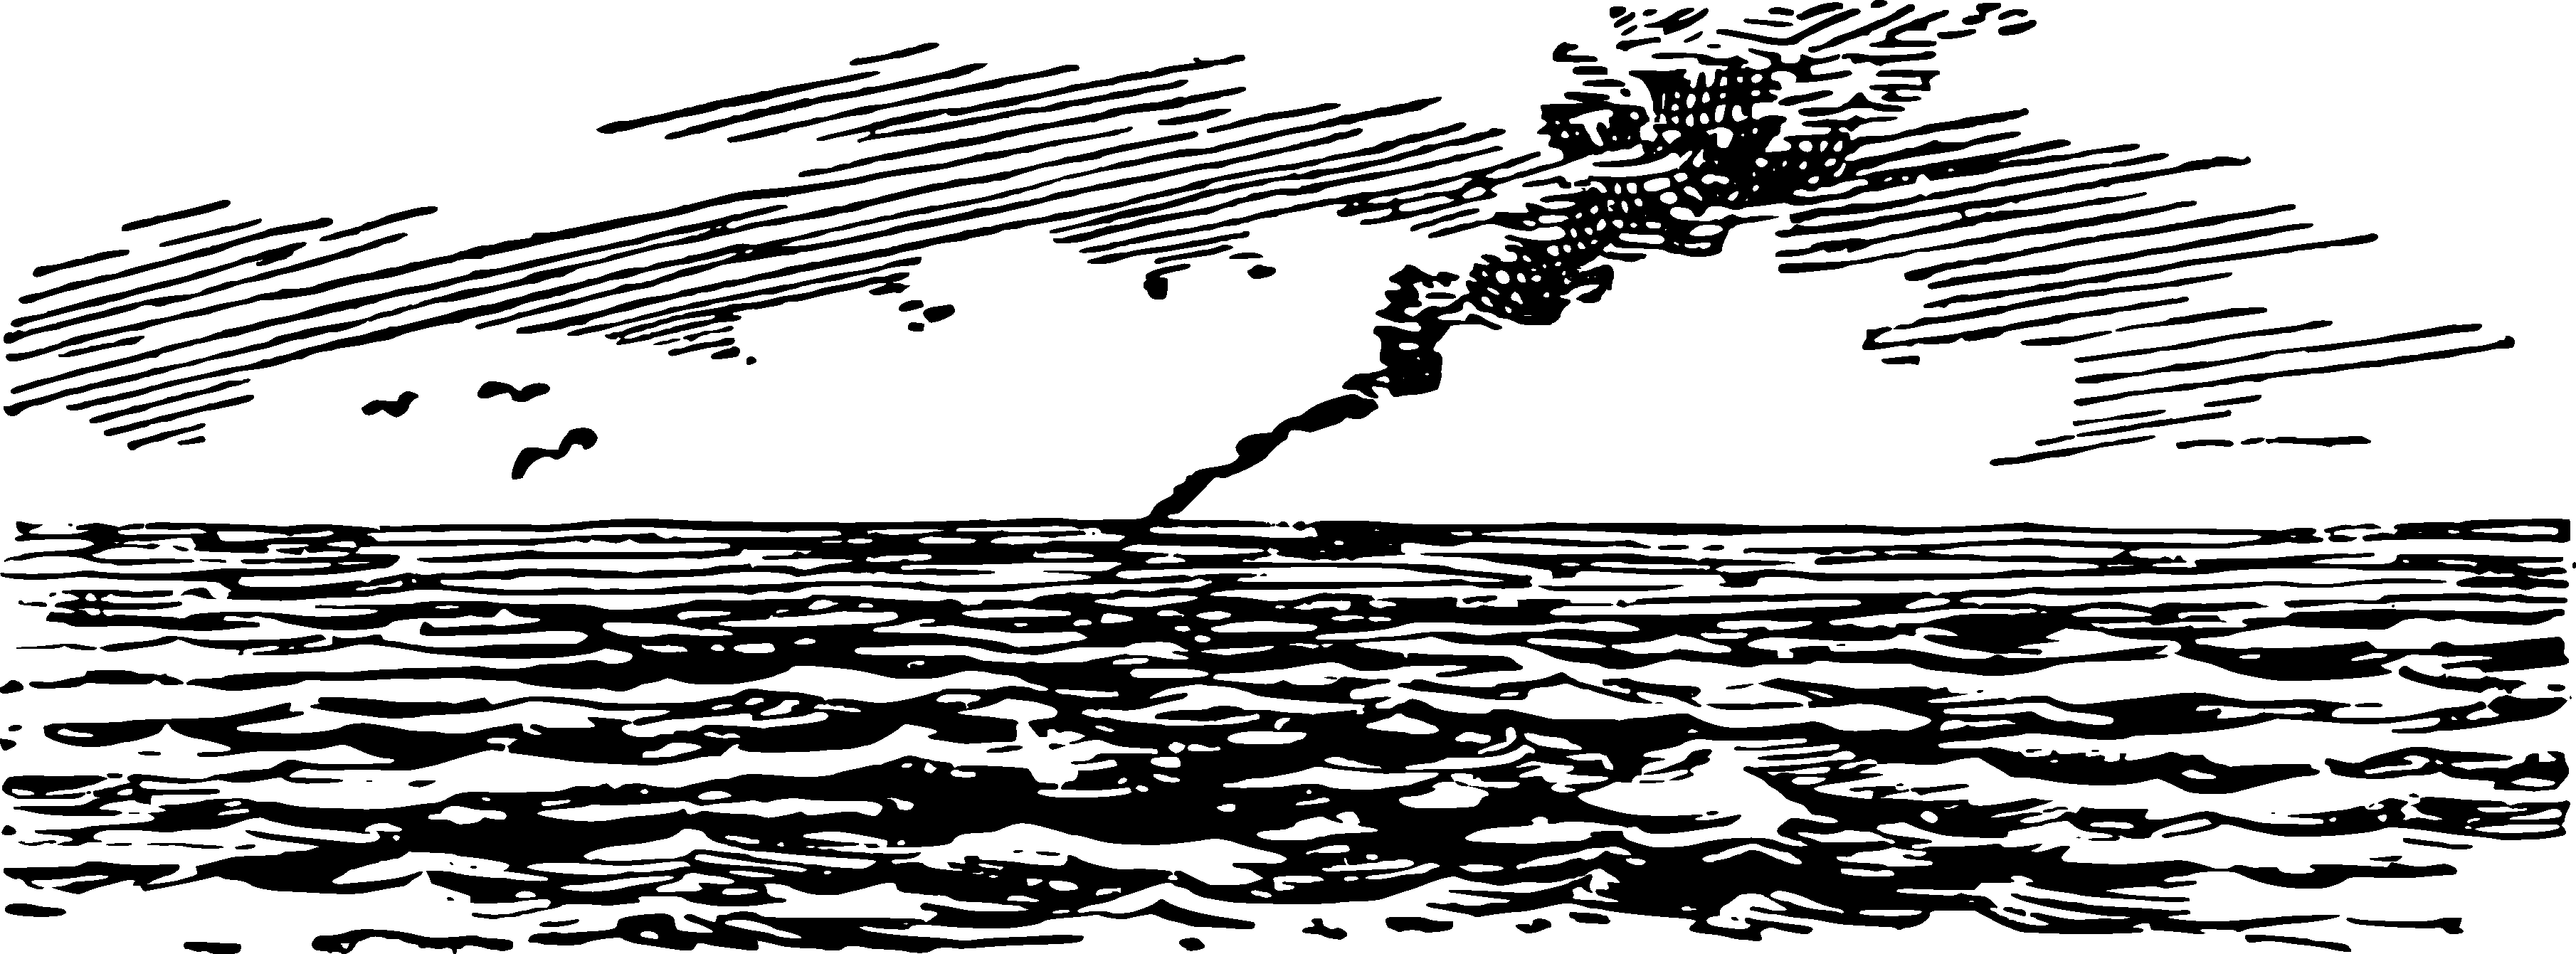
\includegraphics[width=1.2\textwidth]{figures/ch-06/fig-ch-06-head.pdf}\bigskip}

\chapter{Where Heaven and Earth Converge}
\label{ch-06}



	
\section{Horizon}
\label{sec-6.1}
In the countryside or on a level field, you see yourself at the centre of a circle that bounds the earth's surface visible to your eye. This is the \emph{horizon}. The horizon line is elusive: as you approach it, it recedes from you. Yet, although inaccessible, it still exists in reality; it is not an optical illusion or a mirage. For every point of observation, there is a definite boundary of the earth's surface visible from it, and the distance to this boundary is easy to calculate. 

\begin{figure}[h!]
\centering
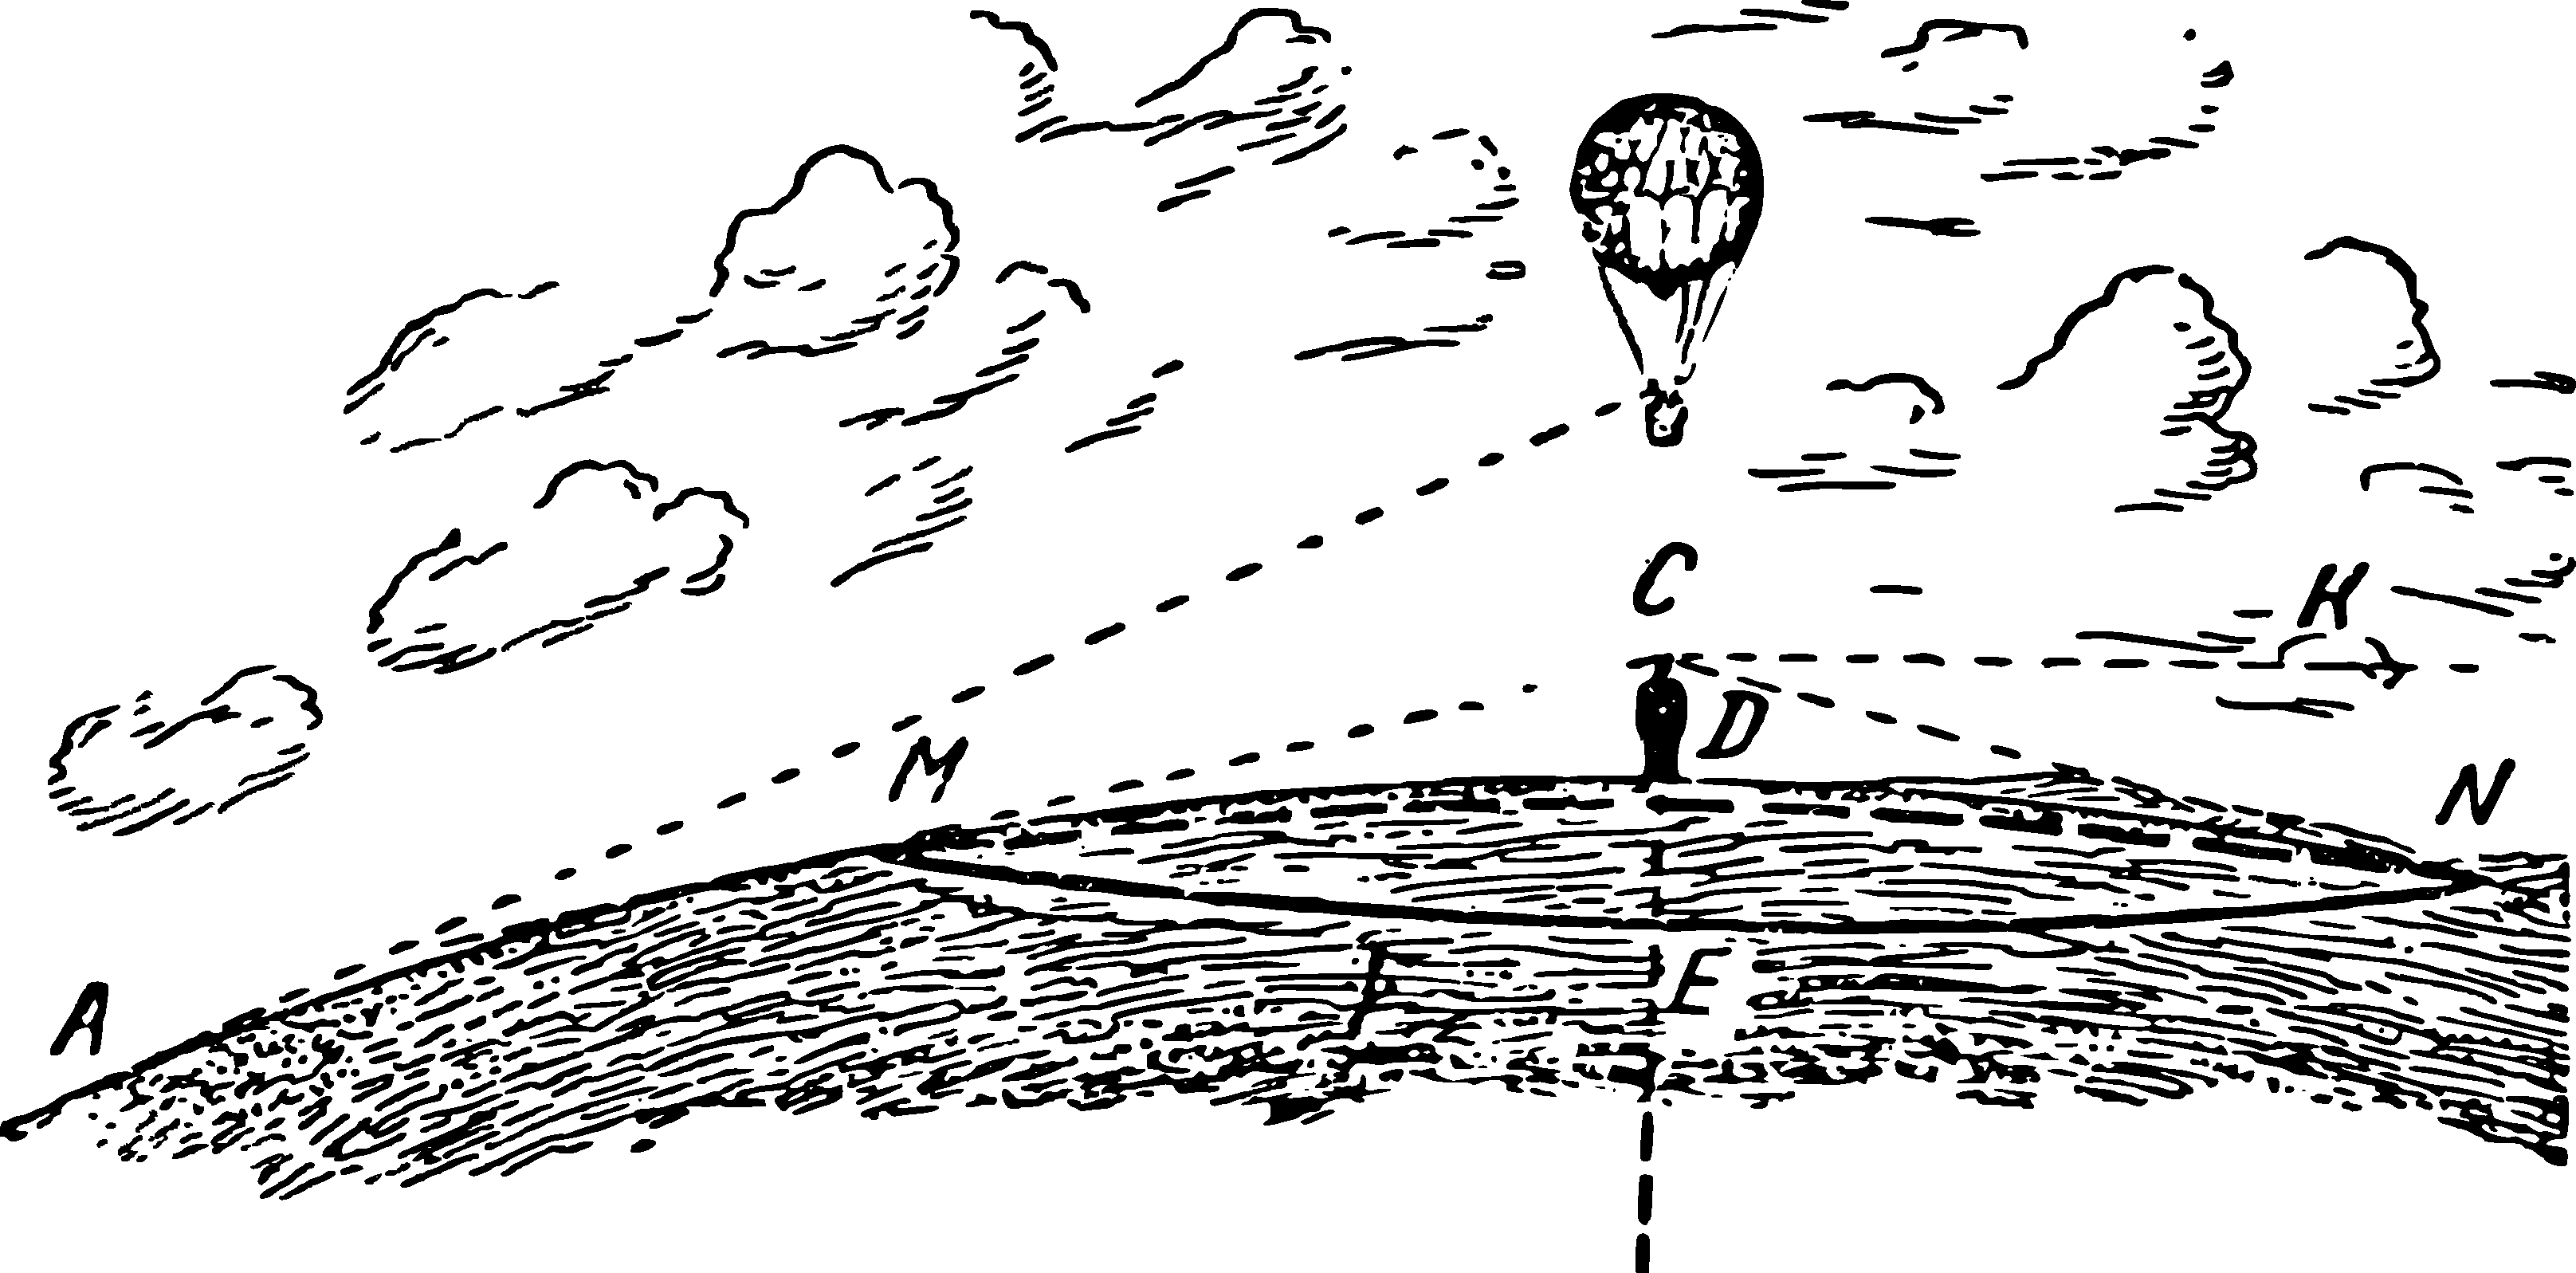
\includegraphics[width=0.9\textwidth]{figures/ch-06/fig-098.pdf}
\sidecaption{The horizon and its dependence on the height of the observation.\label{fig-098}}
\end{figure}

To understand the geometric relationships associated with the horizon, let's refer to \figr{fig-098}, depicting a portion of the earth. At point $C$, the observer's eye is placed at a height $CD$ above the earth's surface. How far does this observer see around them on a level surface? Obviously, only to points $M$ and $N$, where the line of sight touches the earth's surface: beyond this, the earth lies below the line of sight. These points $M$, $N$ (and others lying on the circle $MEN$) represent the boundary of the visible part of the earth's surface, i.e. they form the horizon line. The observer must feel as though the sky meets the earth here because at these points, they simultaneously see both the sky and earthly objects.

Perhaps you might think that \figr{fig-098} does not give an accurate depiction of reality: after all, in reality, the horizon always remains at eye level, whereas in the illustration, the circle clearly lies below the observer. Indeed, we always perceive the horizon line to be at the same level as our eyes and even rising with us as we ascend. But this is an optical illusion: in reality, the horizon line is always below the eye, as shown in \figr{fig-098}. However, the angle formed by the straight lines $CN$ and $CM$ with the line $CK$, perpendicular to the radius at point $C$ (this angle is called the `dip of the horizon'), is very small, and it is impossible to perceive it without instruments.

Incidentally, let's note another interesting circumstance. We just mentioned that when the observer is raised above the earth's surface, for example, in an aeroplane, the horizon line seems to remain at eye level, i.e., it appears to rise with the observer. If one ascends high enough, it will seem as if the ground beneath the aeroplane lies below the horizon line -- in other words, the earth appears concave, with the horizon line serving as its edges. This is well described and explained by Edgar Allan Poe in the fantastical `The Balloon-Hoax'.

\begin{figure}[h!]
\centering
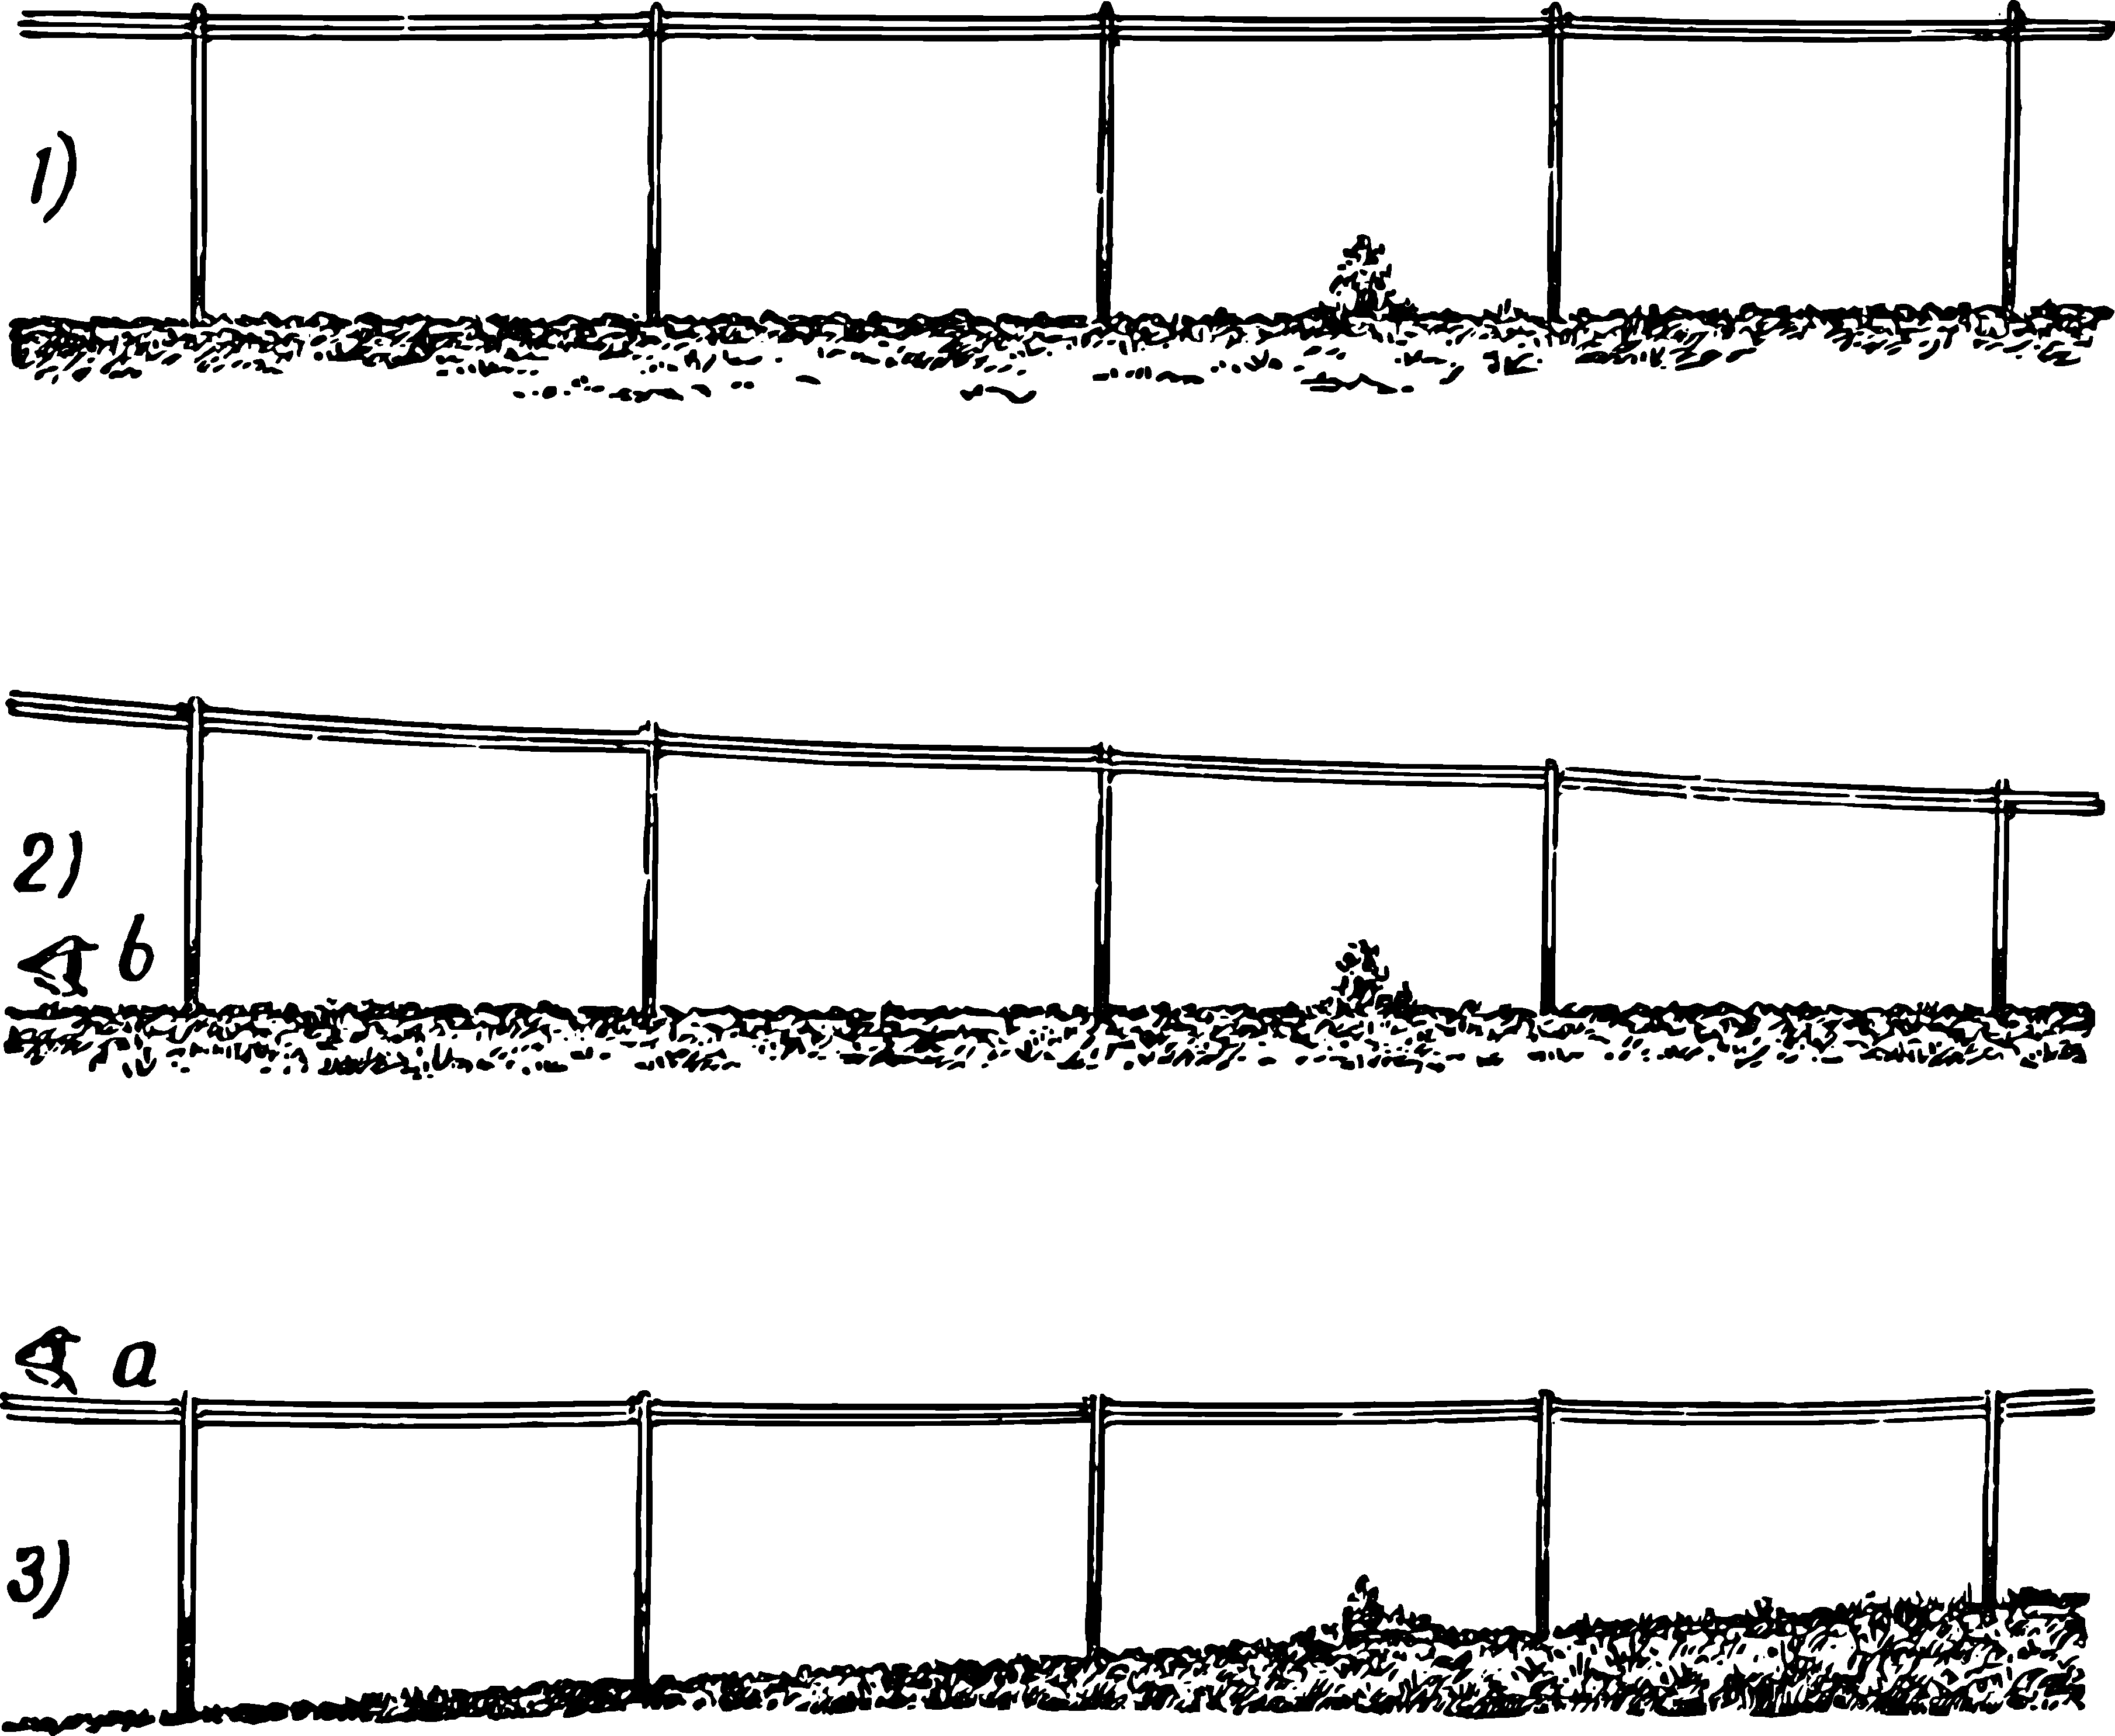
\includegraphics[width=0.9\textwidth]{figures/ch-06/fig-099.pdf}
\sidecaption{What does an eye observing the row of telegraph poles see?\label{fig-099}}
\end{figure}

``More than anything else,'' his aeronaut hero recounts, ``I was astonished by the circumstance that the surface of the earth seemed concave. I expected to see it convex during ascent; only through reflection did I find an explanation for this phenomenon. A plumb-line drawn from my balloon to the earth would form the cathetus of a right triangle, the base of which would be the line from the base of the plumb to the horizon, and the hypotenuse would be the line from the horizon to my balloon. But my height was insignificant compared to the field of view; in other words, the base and hypotenuse of the imaginary right triangle were so great compared to the plumb-line cathetus that they could be considered almost parallel. Therefore, every point directly beneath the aeronaut always seems to lie below the horizon level. Hence the impression of concavity. And this should continue until the height of ascent becomes so significant that the base of the triangle and the hypotenuse cease to appear parallel.''



In addition to this explanation, let's add the following example. Imagine a straight row of telegraph poles (\figr{fig-099}). For an eye placed at point $b$, at the level of the bases of the poles, the row appears as indicated by the number $\mathit{2}$. But for an eye at point $a$, at the level of the tops of the poles, the row appears as $\mathit{3}$, i.e., the ground seems to him as if rising at the horizon.


\section{Ship on the Horizon}
\label{sec-6.2}

When we observe a ship from the shore of the sea or a large lake, emerging from below the horizon, it seems to us that we see the vessel not at the point (\figr{fig-100}) where it actually is, but much closer, at point $B$, where our line of sight glides over the convexity of the sea. When observed with the naked eye, it is difficult to shake the impression that the ship is at point $B$, rather than farther beyond the horizon (compare with what was said in the fourth chapter about the influence of a hill on judging distance).

\begin{figure}[h!]
\centering
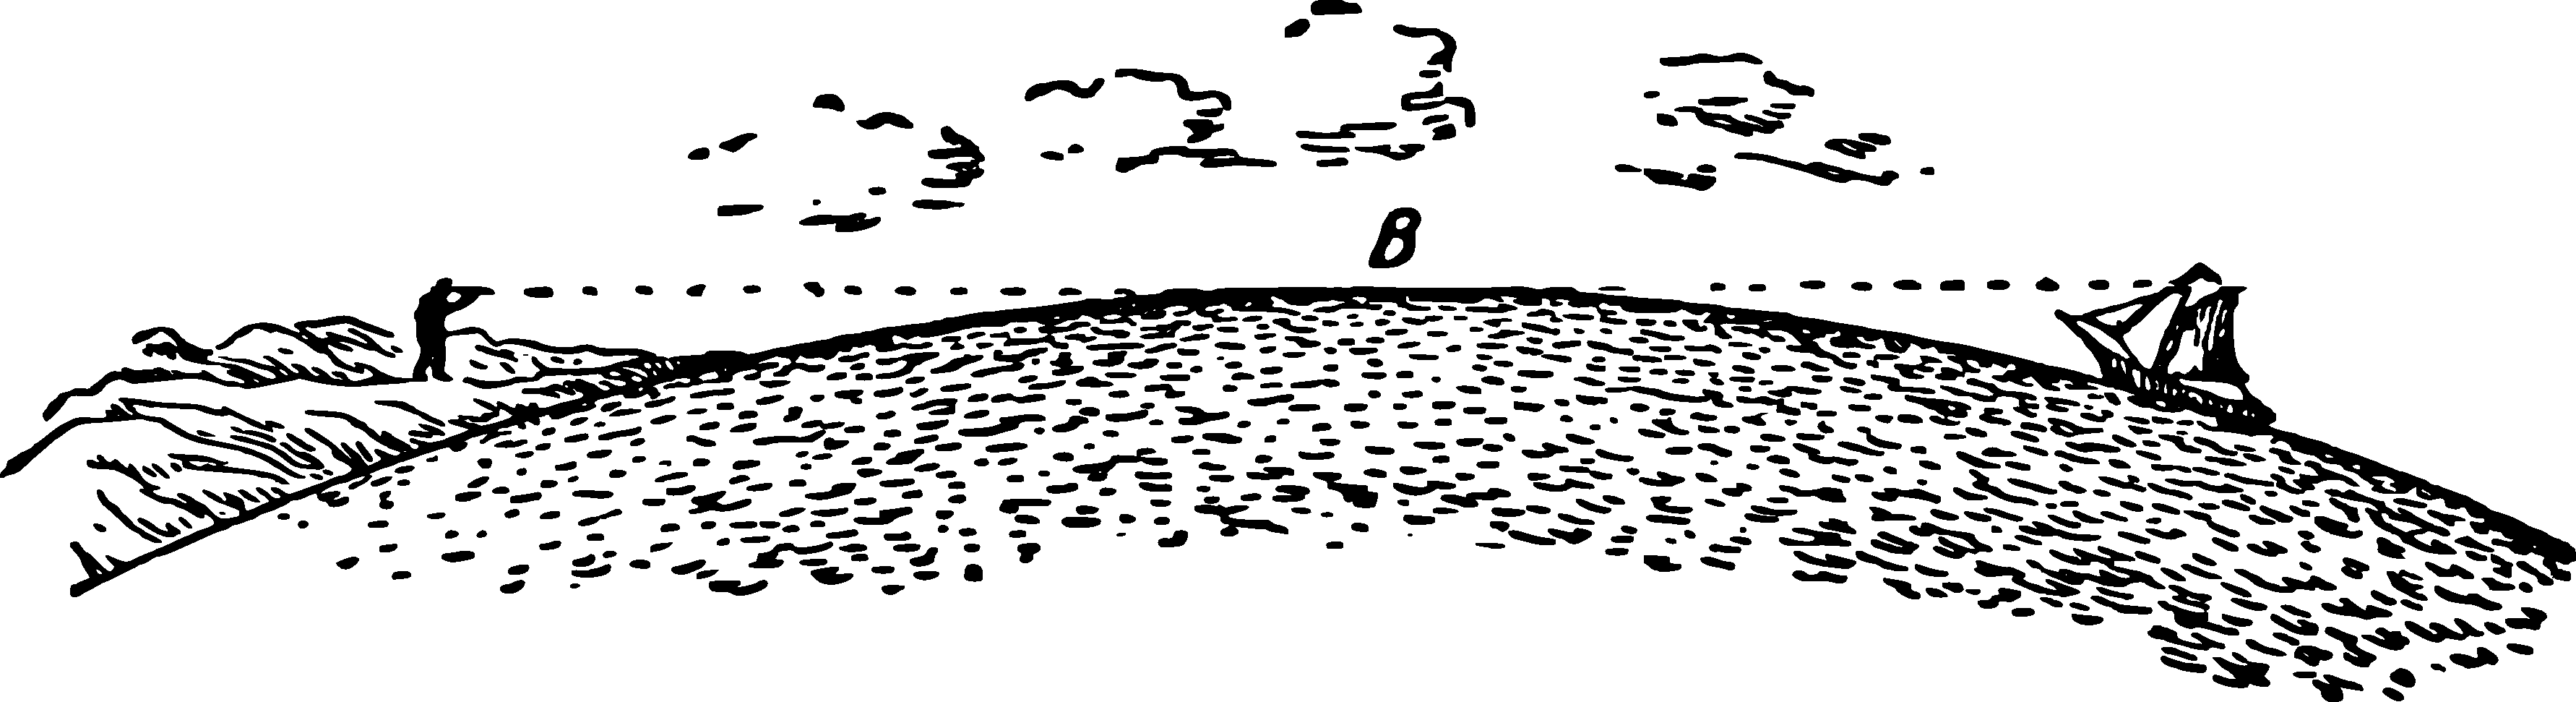
\includegraphics[width=0.9\textwidth]{figures/ch-06/fig-100.pdf}
\sidecaption{Ship beyond the horizon.\label{fig-100}}
\end{figure}

However, through a telescope, this different distance of the ship is perceived much more distinctly. The telescope does not show objects nearby and far away equally clearly: through a telescope aimed into the distance, nearby objects appear blurred, and conversely, a telescope aimed at nearby objects shows distant ones in a haze. Therefore, if one directs a telescope (with sufficient magnification) at the water's horizon and adjusts it so that the water surface is clearly visible, the ship will appear in blurred outlines, revealing its greater distance from observation (\figr{fig-101}). Conversely, setting the telescope to sharply show the outlines of the ship, partially hidden below the horizon, we will notice that the water surface at the horizon loses its previous clarity and appears as if in a haze (\figr{fig-102}).

\begin{figure}[h!]
\centering
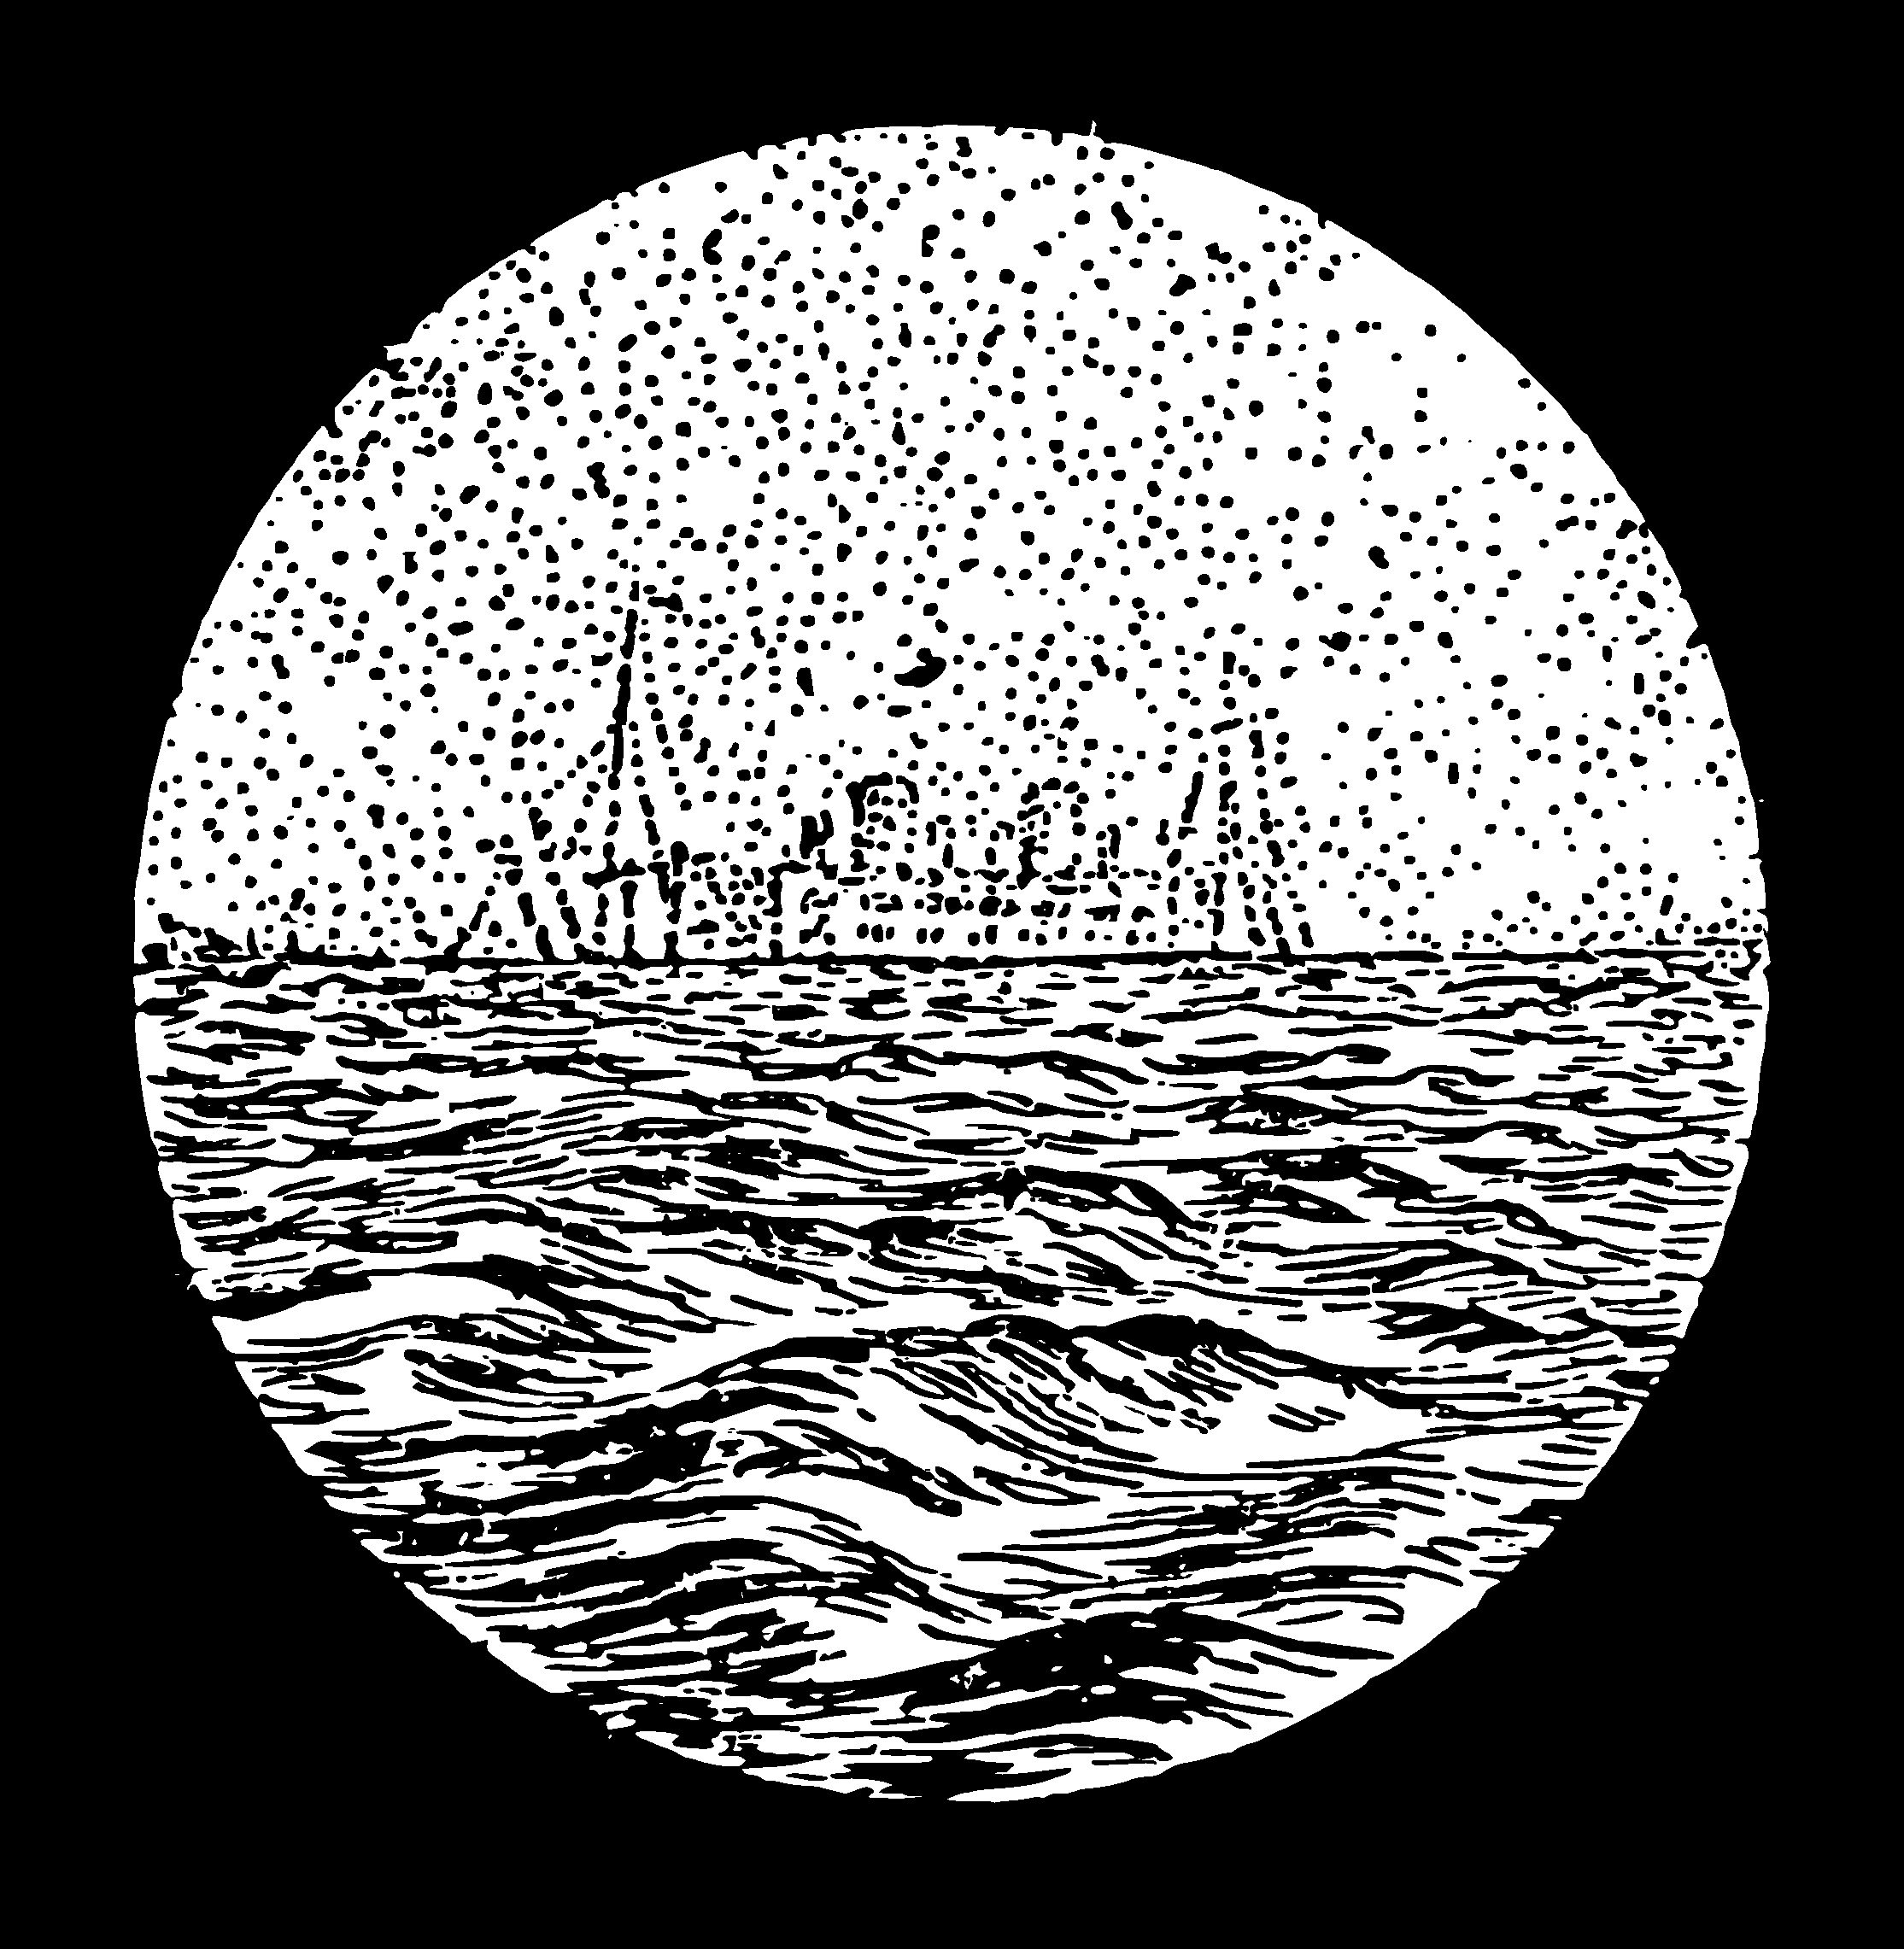
\includegraphics[width=0.55\textwidth]{figures/ch-06/fig-101.pdf}
\sidecaption{A ship over the horizon, viewed through a telescope with focus on water surface.\label{fig-101}}
\end{figure}

\begin{figure}[h!]
\centering
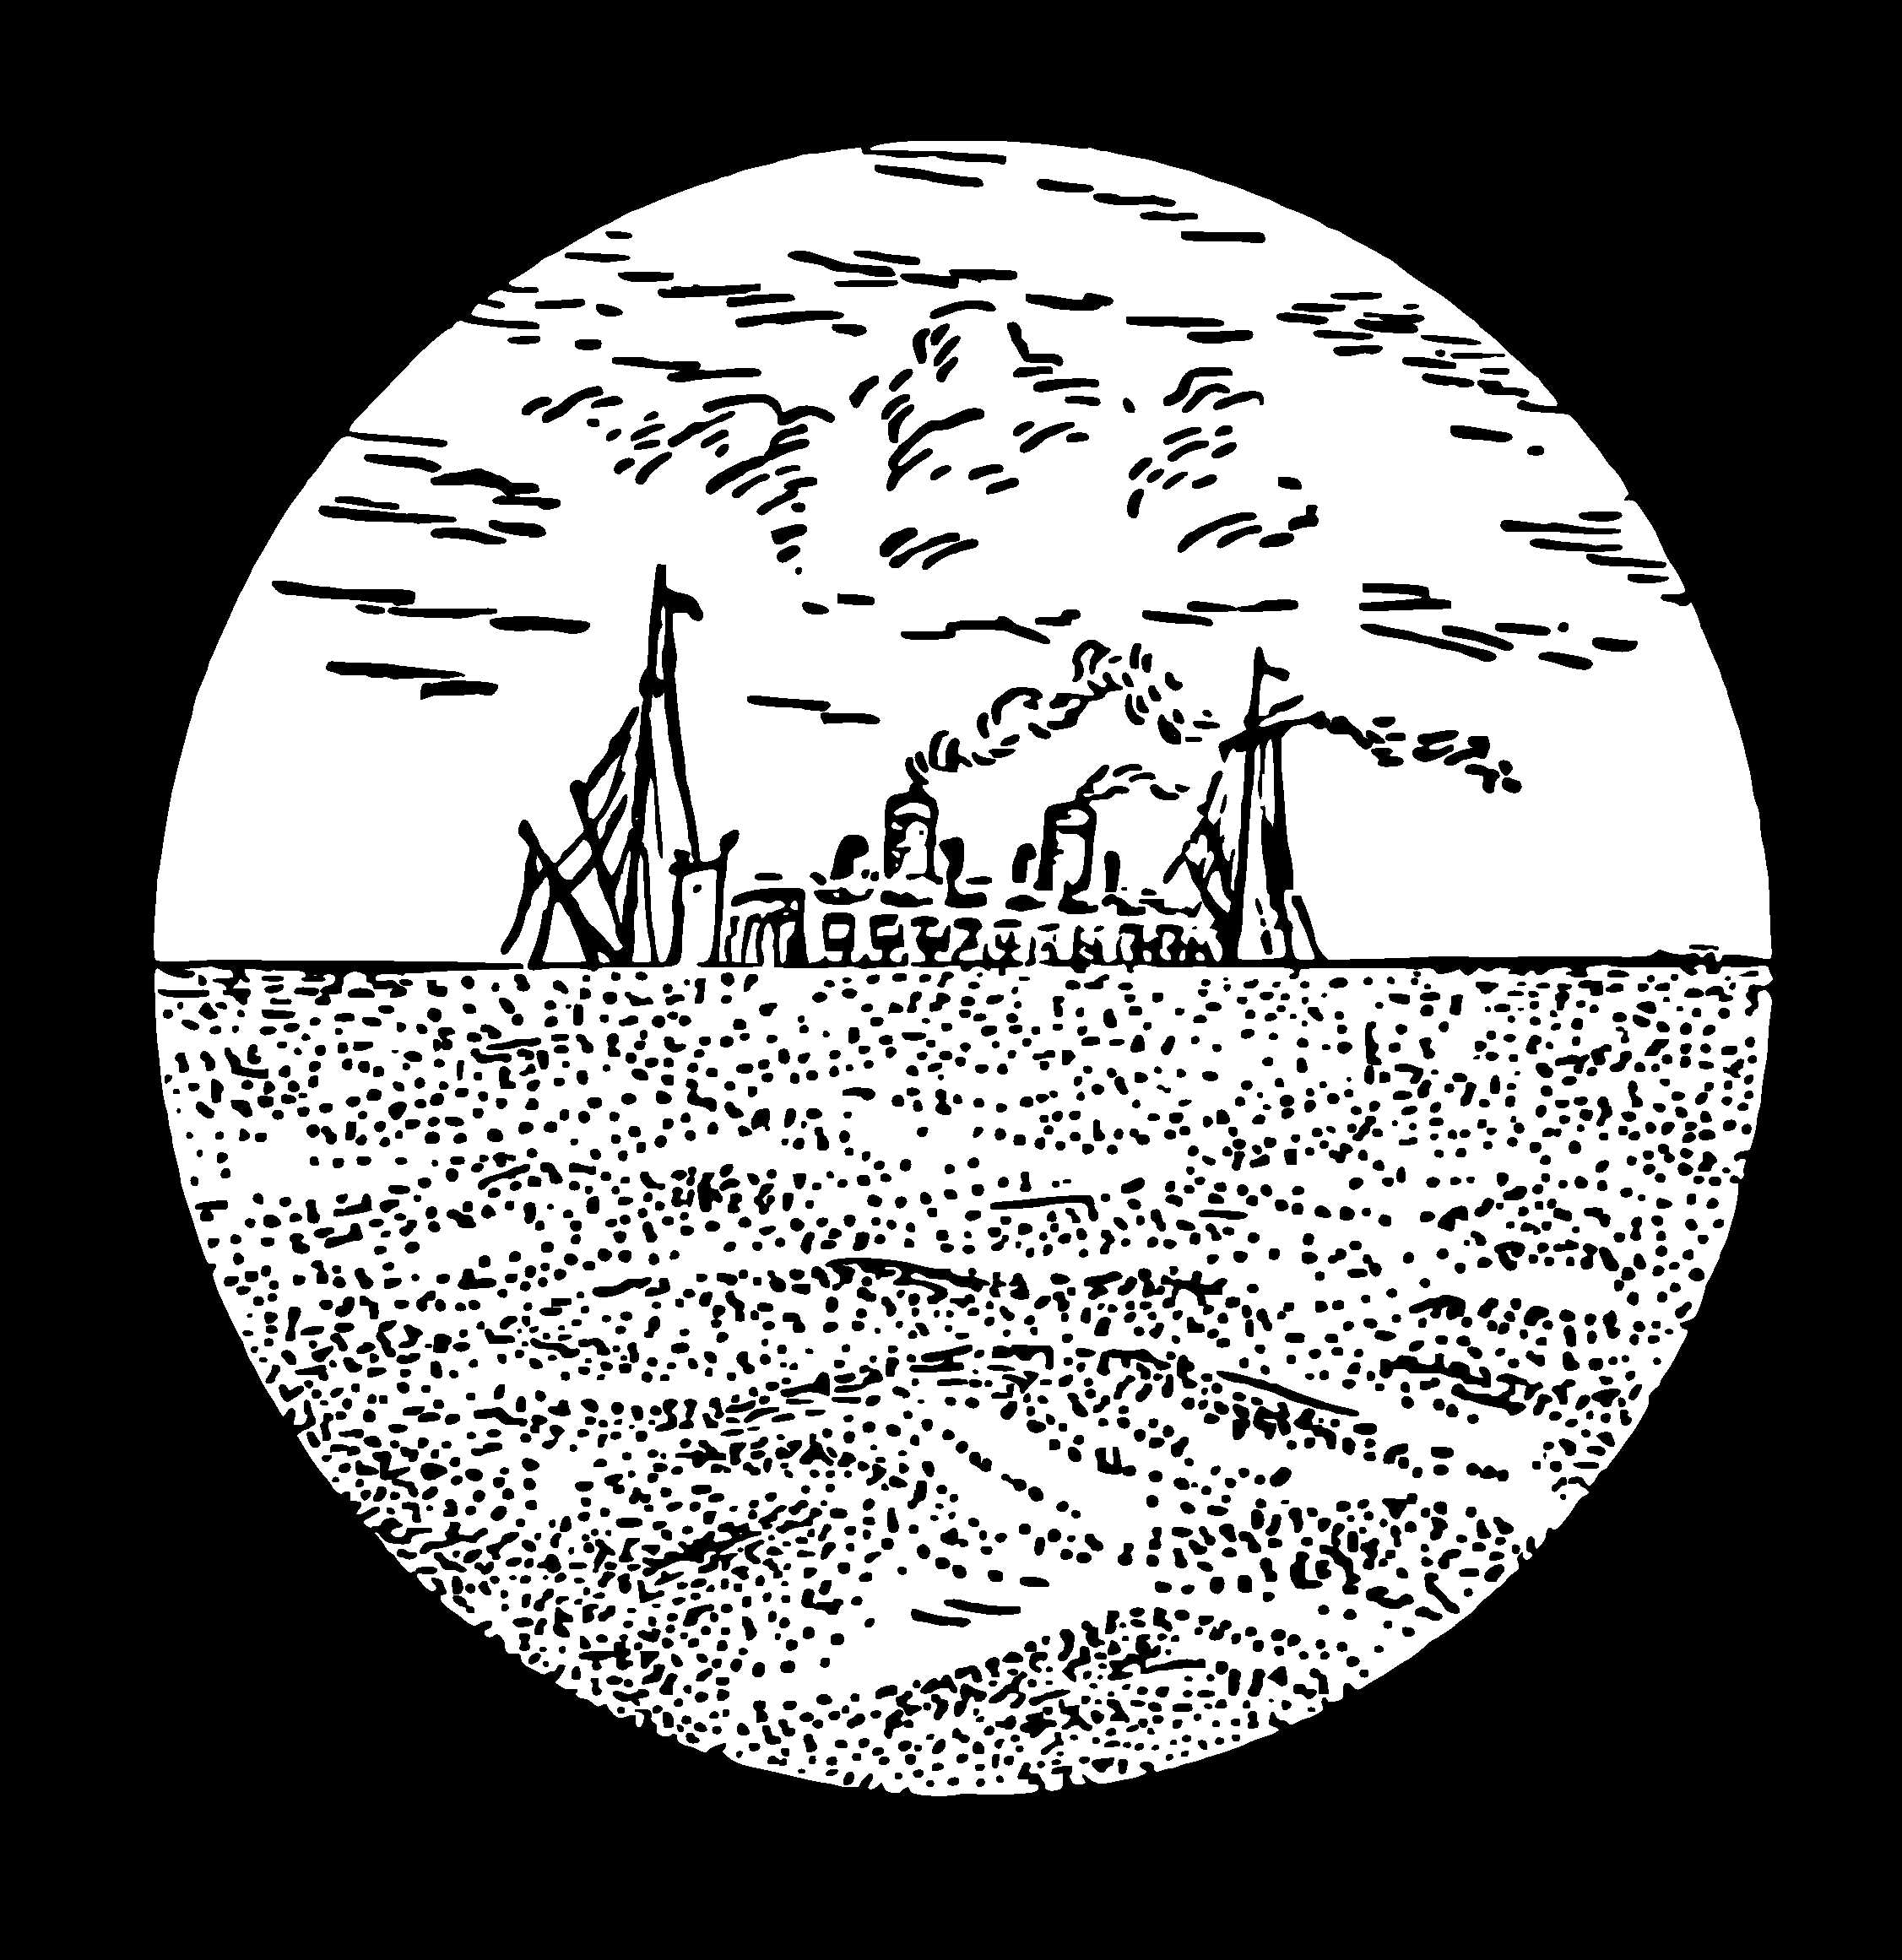
\includegraphics[width=0.55\textwidth]{figures/ch-06/fig-102.pdf}
\sidecaption{A ship over the horizon, viewed through a telescope with focus on the ship.\label{fig-102}}
\end{figure}

\section{The Distance to the Horizon}
\label{sec-6.3}

How far does the horizon line lie from the observer? In other words, what is the radius of the circle centred around ourselves on level ground? How to calculate the distance to the horizon, knowing the elevation of the observer above the earth's surface?

\begin{figure}[h!]
\centering
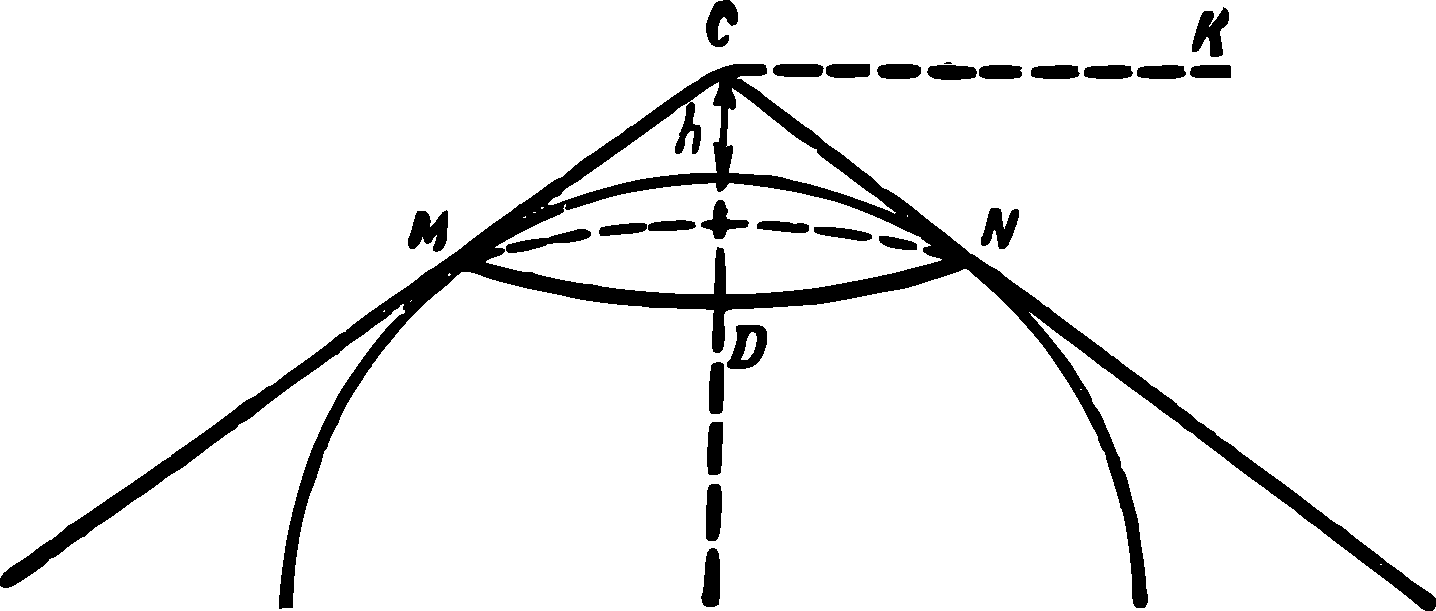
\includegraphics[width=0.8\textwidth]{figures/ch-06/fig-103.pdf}
\sidecaption{The problem of the distance to the horizon.\label{fig-103}}
\end{figure}

The problem boils down to calculating the length of segment $CN$ (\figr{fig-103}), the tangent drawn from the observer's eye to the earth's surface. The square of the tangent -- as we know from geometry -- equals the product of the external segment $h$ by the secant to the entire length of this secant, i.e., by $h + 2R$, where $R$ is the radius of the earth. Since the elevation of the observer's eye above the ground is usually extremely small compared to the diameter ($2R$) of the earth, for example, for the highest altitude of an aeroplane, it is about 0.001 of its fraction, then $h + 2R$  can be taken as approximately 2R, and then the formula simplifies to:
\begin{equation*}%
CN^{2} = h 2R.
\end{equation*}
Therefore, the distance to the horizon can be calculated by a very simple formula:
\begin{equation*}%
\text{distance to the horizon} = \sqrt{2Rh},
\end{equation*}
where $R$ is the radius of the earth (about \SI{6400}{\kilo\meter}\sidenote{More precisely, 6371 km.}), and $h$ is the elevation of the observer's eye above the earth's surface.

Since $\sqrt{6400} = 80$, the formula can be expressed as follows:
\begin{equation*}%
\text{distance to the horizon} = 80\sqrt{2h} = 113\sqrt{h},
\end{equation*}
where $h$ should be expressed in kilometres.

This calculation is purely geometrical and simplified. If we wish to refine it considering physical factors influencing the distance to the horizon, we must take into account the so-called `atmospheric refraction'. Refraction, i.e., the bending of light rays in the atmosphere, increases the distance to the horizon by approximately 1/15 of the calculated distance (by about 6\%). The number 6\% is just an average. The distance to the horizon is slightly increased or decreased depending on many conditions, namely:

\begin{footnotesize}
\begin{center}
\begin{tabular}{p{3cm}p{3cm}}
\toprule
\textbf{Increases} & \textbf{Decreases} \\
\midrule
 at high pressure, &  at low pressure,\\
 near the Earth's surface, & at heights,\\
 in cold weather, & in warm weather,\\
 in the morning and evening, & during the day,\\
 in humid weather, & in dry weather,\\
 over the sea, & over land.\\
\bottomrule
\end{tabular}
\end{center}
\end{footnotesize}



\ques How far can a person standing on a plain see the earth? 

\ans Assuming that the eyes of an adult are elevated by 1.6 meters, or 0.0016 km, we have:
\begin{equation*}%
\text{distance to the horizon} = 113 \times \sqrt{0.0016} = \SI{4.52}{\kilo\meter}.
\end{equation*}
The Earth's atmosphere, as mentioned earlier, bends the path of rays, causing the horizon to recede on average by 6\%. Further than that distance obtained by the formula. To account for this correction, we need to multiply \SI{4.52}{\kilo\meter} by 1.06; we get: 
\begin{equation*}%
4.52 \times 1.06 = \SI{4.8}{\kilo\meter}.
\end{equation*}
Thus, a person of average height can see no further than \SI{4.8}{\kilo\meter} on a level surface. The diameter of the circle he observes is only \SI{9.6}{\kilo\meter}, and the area is \SI{72}{\kilo\meter\squared}. This is much less than what people usually think when they describe the distant expanse of the steppes, scanned by the eye.



\ques How far can a person sitting in a boat see the sea?

\ans If we assume that the elevation of the eyes of a person sitting in a boat above the water level is 1 meter, or \SI{0.001}{\kilo\meter}, then the distance to the horizon is approximately 
\begin{equation*}%
113 \sqrt{0.001} = \SI{3.58}{\kilo\meter},
\end{equation*} 
or considering the average atmospheric refraction, about \SI{3.8}{\kilo\meter}. Objects located farther away are visible only in their upper parts; their bases are hidden below the horizon.

At a lower position of the eye, the horizon narrows: for half a meter, for example, up to \SI{2}{\kilo\meter}. On the contrary, when observed from elevated points (from the mast), the horizon range increases: for \SI{4}{\meter}, for example, up to \SI{7}{\kilo\meter}.

\ques How far in all directions did the land stretch for the aviators observing from the gondola of the stratosphere balloon \emph{SOAK-1} when it was at the highest point of its ascent?

\ans Since the balloon was at a height of \SI{22}{\kilo\meter}, the horizon distance for such an elevation is:
\begin{equation*}%
113 \sqrt{22} = \SI{530}{\kilo\meter},
\end{equation*}
and with refraction considered -- \SI{580}{\kilo\meter}.

\ques How high should a pilot ascend to see a 50 km radius around themselves?

\ans From the horizon distance formula, in this case, we have the equation:
\begin{align*}%
50 & = 113 \sqrt{2Rh}, \text{Hence, solving for} \,\,h,\\
h & = \frac{50^{2}}{2R} = \frac{2500}{12800} = \SI{0.2}{\kilo\meter}.
\end{align*}
So, it's enough to ascend only \SI{200}{\meter}.

To account for the correction, subtracting 6\% of \SI{50}{\kilo\meter}, we get \SI{47}{\kilo\meter}:
\begin{equation*}%
h = \frac{47^{2}}{2R} = \frac{2200}{12800} = \SI{0.17}{\kilo\meter}.
\end{equation*}
So, approximately \SI{170}{\meter} (instead of 200).
\begin{figure}[h!]
\centering
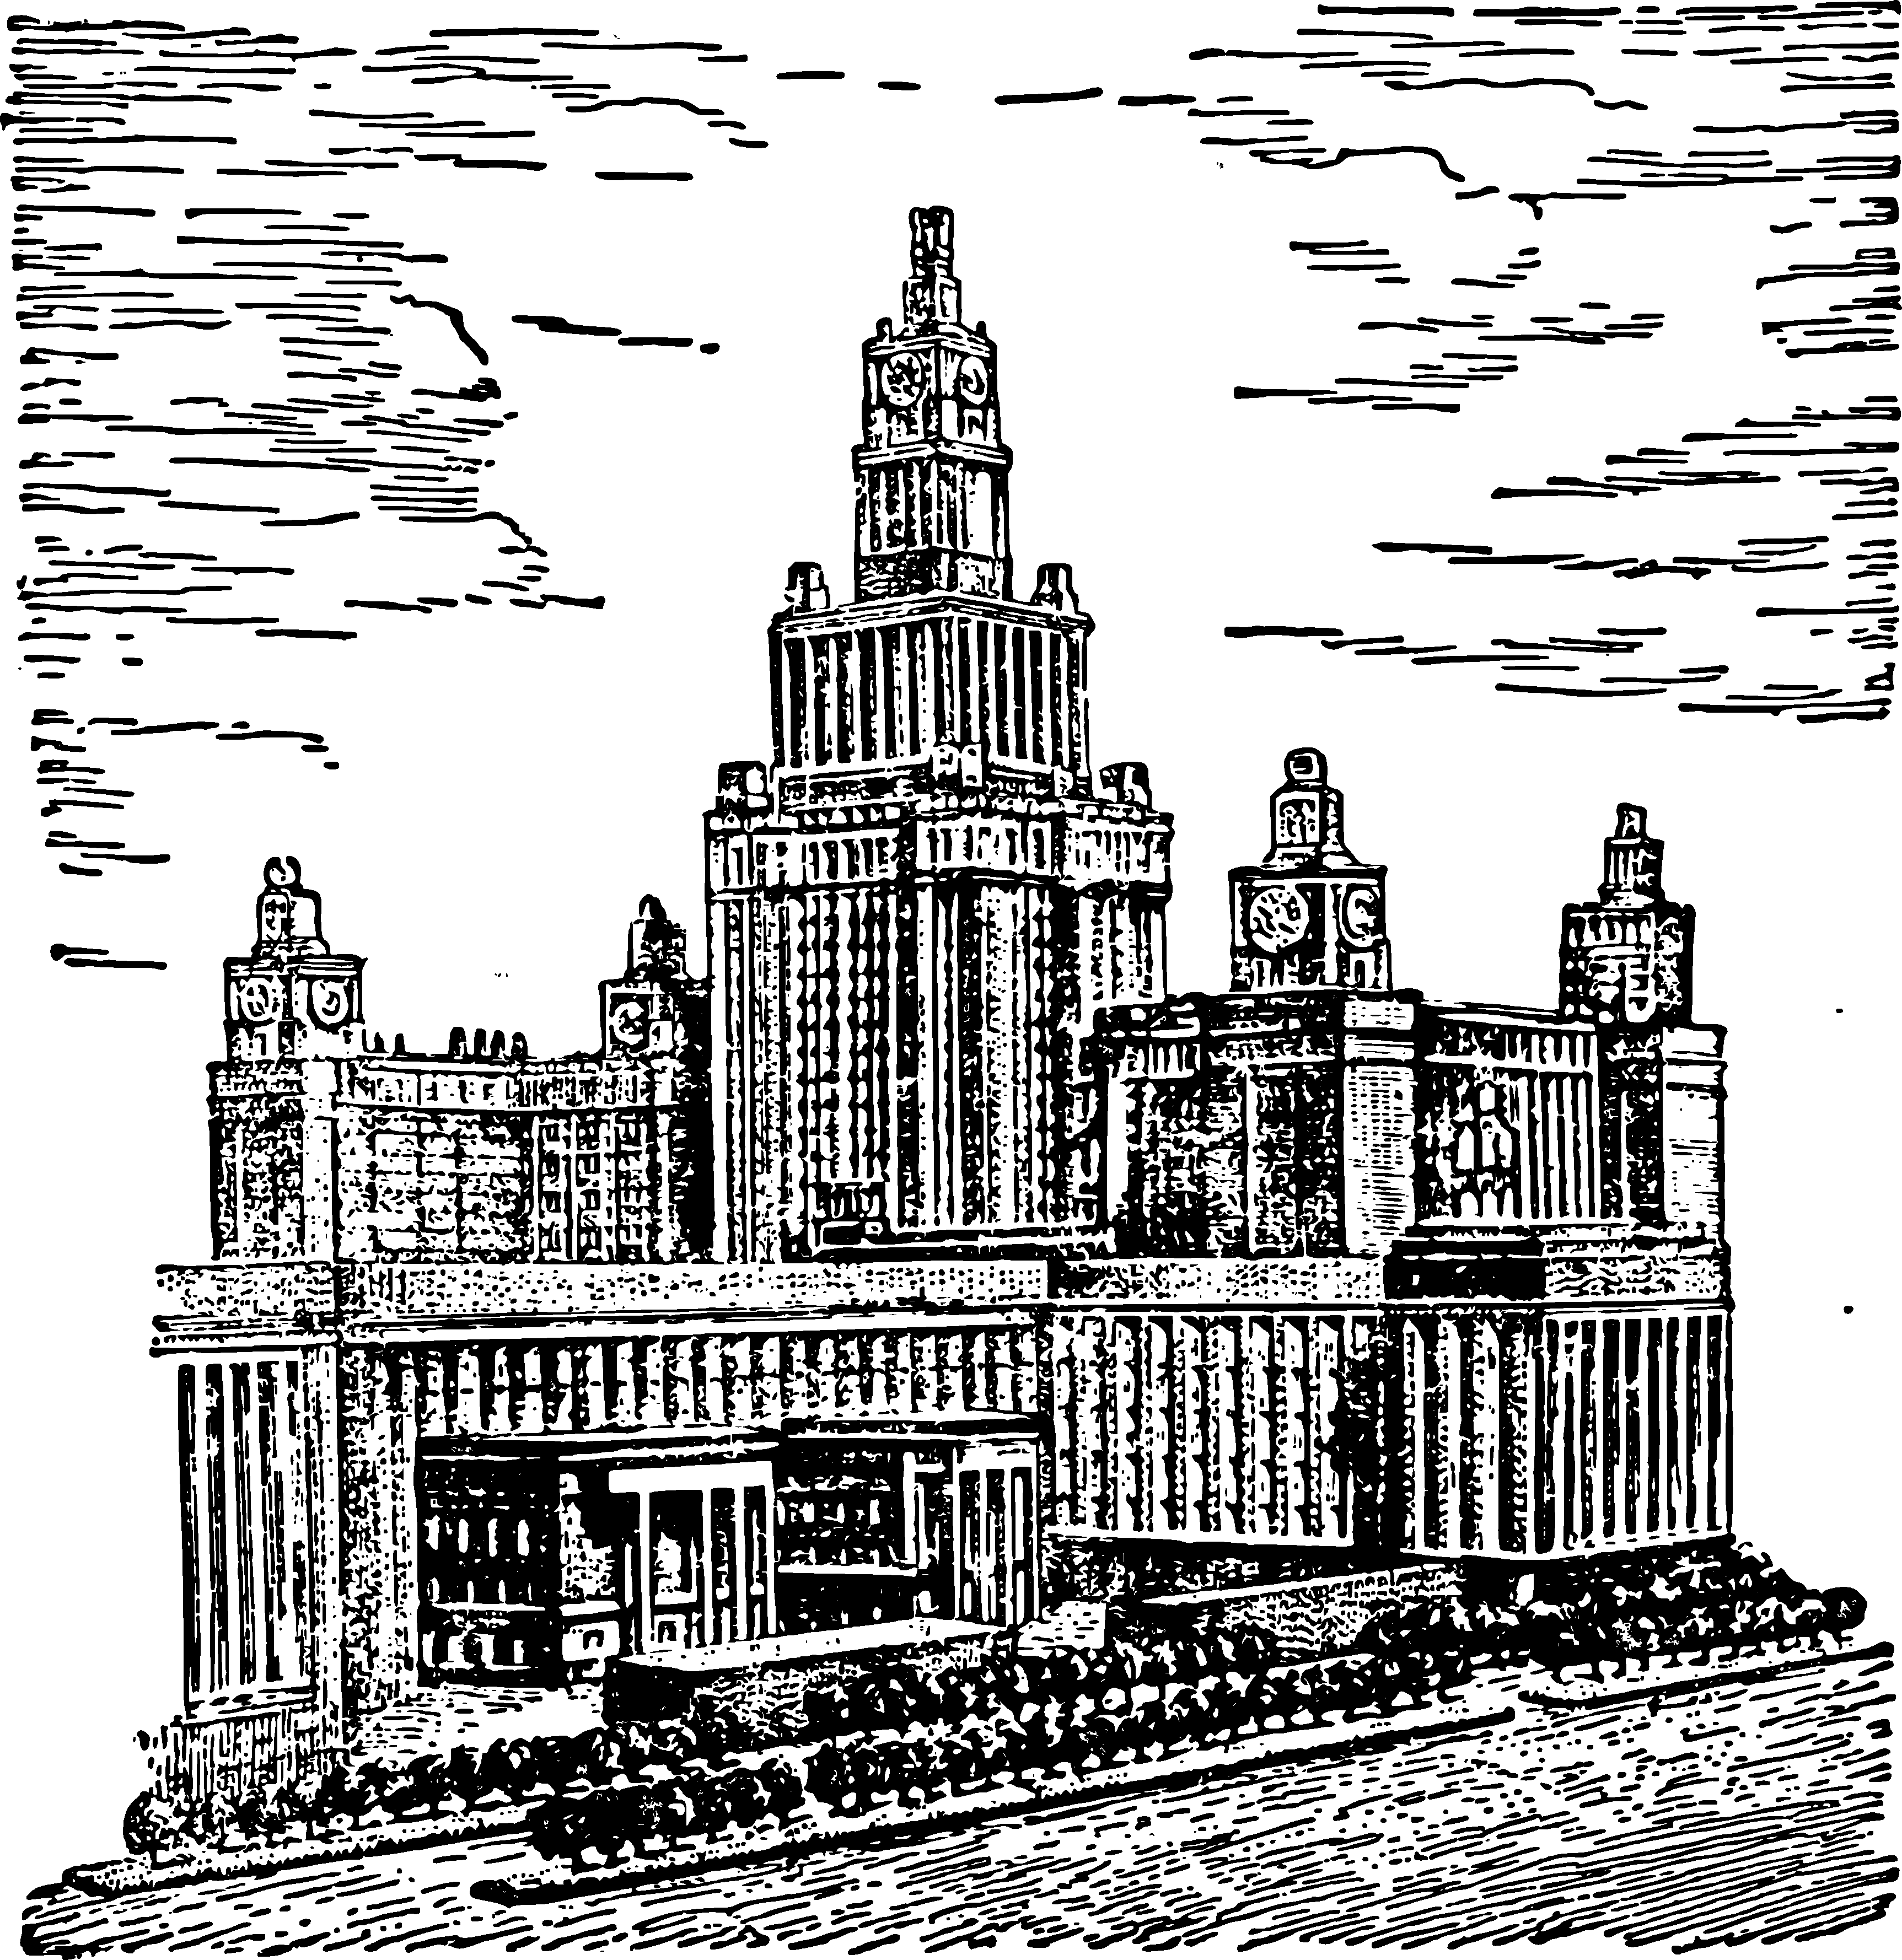
\includegraphics[width=0.8\textwidth]{figures/ch-06/fig-104.pdf}
\sidecaption{Moscow University (drawing from the project of the building under construction).\label{fig-104}}
\end{figure}


The twenty-six-story building of the University (\figr{fig-104}) — the world's largest educational and scientific centre -- is being constructed at the highest point of the Lenin Hills in Moscow.

It will rise \SI{200}{\meter} above the level of the Moscow River.

Therefore, from the windows of the upper floors of the University, a panorama up to \SI{50}{\kilo\meter} in radius will be visible.

\clearpage

\section{Gogol's Tower Problem}
\label{sec-6.4}

It's interesting to know what increases faster: the height of elevation or the horizon distance? Many people think that with the elevation of the observer, the horizon increases extraordinarily fast. This was also thought by Gogol, who wrote in his article \emph{On the Architecture of Our Time}:

\begin{quote}
Huge, colossal towers are necessary in the city\dots{} Here we usually limit them to a height that allows for viewing only the city, whereas for a capital, it is necessary to see, at least, a hundred and fifty versts\sidenote{1 verst is 1.0668 \si{\kilo\meter}; 150 versts $\sim$ \SI{160}{\kilo\meter}.} in all directions, and for this, perhaps just one or two extra floors -- and everything changes. The volume of the horizon expands extraordinarily with elevation.
\end{quote}

Is this really the case?

\ans It's enough to look at the formula 
\begin{equation*}%
\text{horizon distance} = \sqrt{2Rh}, 
\end{equation*}
to immediately understand the fallacy of the claim that the ``volume of the horizon'' increases very quickly with the elevation of the observer. On the contrary, the horizon distance grows slower than the height of elevation: it is proportional to the square root of the height. When the observer's elevation increases by 100 times, the horizon only moves 10 times further away; when the height becomes 1000 times larger, the horizon only moves 31 times further away. Therefore, it is erroneous to assert that ``just one or two extra floors -- and everything changes''. If two more floors are added to an eight-story building, the horizon distance will increase by $\sqrt{10/8}$, i.e., by 1.1 times -- only by 10\%. Such an addition is hardly noticeable.

As for the idea of constructing a tower from which one could see, ``at least, a hundred and fifty versts,'' i.e., 160 km, it is completely unattainable. Gogol, of course, did not realize that such a tower would have to have an enormous height.

Indeed, from the equation:
\begin{align*}%
160 & = \sqrt{2Rh}, \,\, \text{we get,}\\
h & = \frac{160^{2}}{2R}  = \frac{25600}{12800} = \SI{3268}{\meter}.
\end{align*}
This is the height of a large mountain. The highest of the currently designed buildings in the capital of our Homeland is an 32-story administrative building, the gilded spire of which is planned to rise 280 meters from the base of the building -- seven times lower than the heights envisioned by Gogol.\sidenote[][-2cm]{As of 2024, \emph{Burj Khalifa} in Dubai is the tallest building in the world at \SI{828}{\metre}. The horizon visible from top of this building is equal to $\sqrt{12800 \times 0.828} \approx \SI{93.6}{\kilo\meter}$. -- \textsc{dm}} 


\section{Pushkin's Hill}

Pushkin makes a similar mistake when speaking in \emph{The Covetous Knigh} about the distant horizon opening up from the top of the ``proud hill'':
\begin{quote}
And the king could joyfully behold from the height\\
Both the valley covered with white tents, And the sea, where the ships were running\dots{}
\end{quote}
We have already seen how modest the height of this ``proud'' hill was: even the hordes of Attila could not erect a hill higher than 4.5 meters by this method. Now we can complete the calculations by determining how much this hill expanded the horizon of the observer placed on its peak. The eye of such a spectator would be elevated above the ground by $4.5 + 1.5 = 6$ meters, and therefore, the horizon distance would be 
\begin{equation*}%
\sqrt{2 \times 6400 \times 0.006} = \SI{8.8}{\kilo\meter}.
\end{equation*}
This is only \SI{4}{\kilo\meter} more than what can be seen from standing on flat ground.


\section{Where the Rails Meet}
\label{sec-6.6}

\ques Certainly, you have noticed how the railway tracks narrowing into the distance. But have you ever seen the point where both rails finally meet each other? And is it possible to see such a point? You now have enough knowledge to solve this problem.

\ans Let's remember that each object turns into a point for the normal eye when it is seen at an angle of \ang{;1}, i.e., when it is at a distance of 1/3400 of its diameter. The width of the railway track is \SI{1.52}{\meter}. Therefore, the gap between the rails should merge into a point at a distance of $1.52 \times 3400 = \SI{5.2}{\kilo\meter}$. So, if we could follow the rails for \SI{5.2}{\kilo\meter}, we would see how they both converge at one point. But on flat ground, the horizon lies closer than \SI{5.2}{\kilo\meter}, precisely at a distance of only \SI{4.4}{\kilo\meter}. Therefore, a person with normal vision standing on flat ground cannot see the point where the rails meet. They could only observe it under one of the following conditions:
\begin{enumerate}
\item if their visual acuity is reduced so that objects merge into a point for them at an angle of more than \ang{;1};
\item if the railway track is not horizontal;
\item if the observer's eye is elevated above the ground by more than $5.2^{2}/2R = 27/12800 = 0.0021\si{\kilo\meter}$, i.e., \SI{210}{\centi\meter}.
\end{enumerate}

\section{Lighthouse Problems}
\label{sec-6.7}



\ques There is a lighthouse on the shore, the top of which rises 40 meters above the water's surface.

From what distance will this lighthouse be visible to a sailor-observer (``mastman'') on the ``mast'' of the ship at a height of 10 meters above the water's surface?


\begin{figure}[h!]
\centering
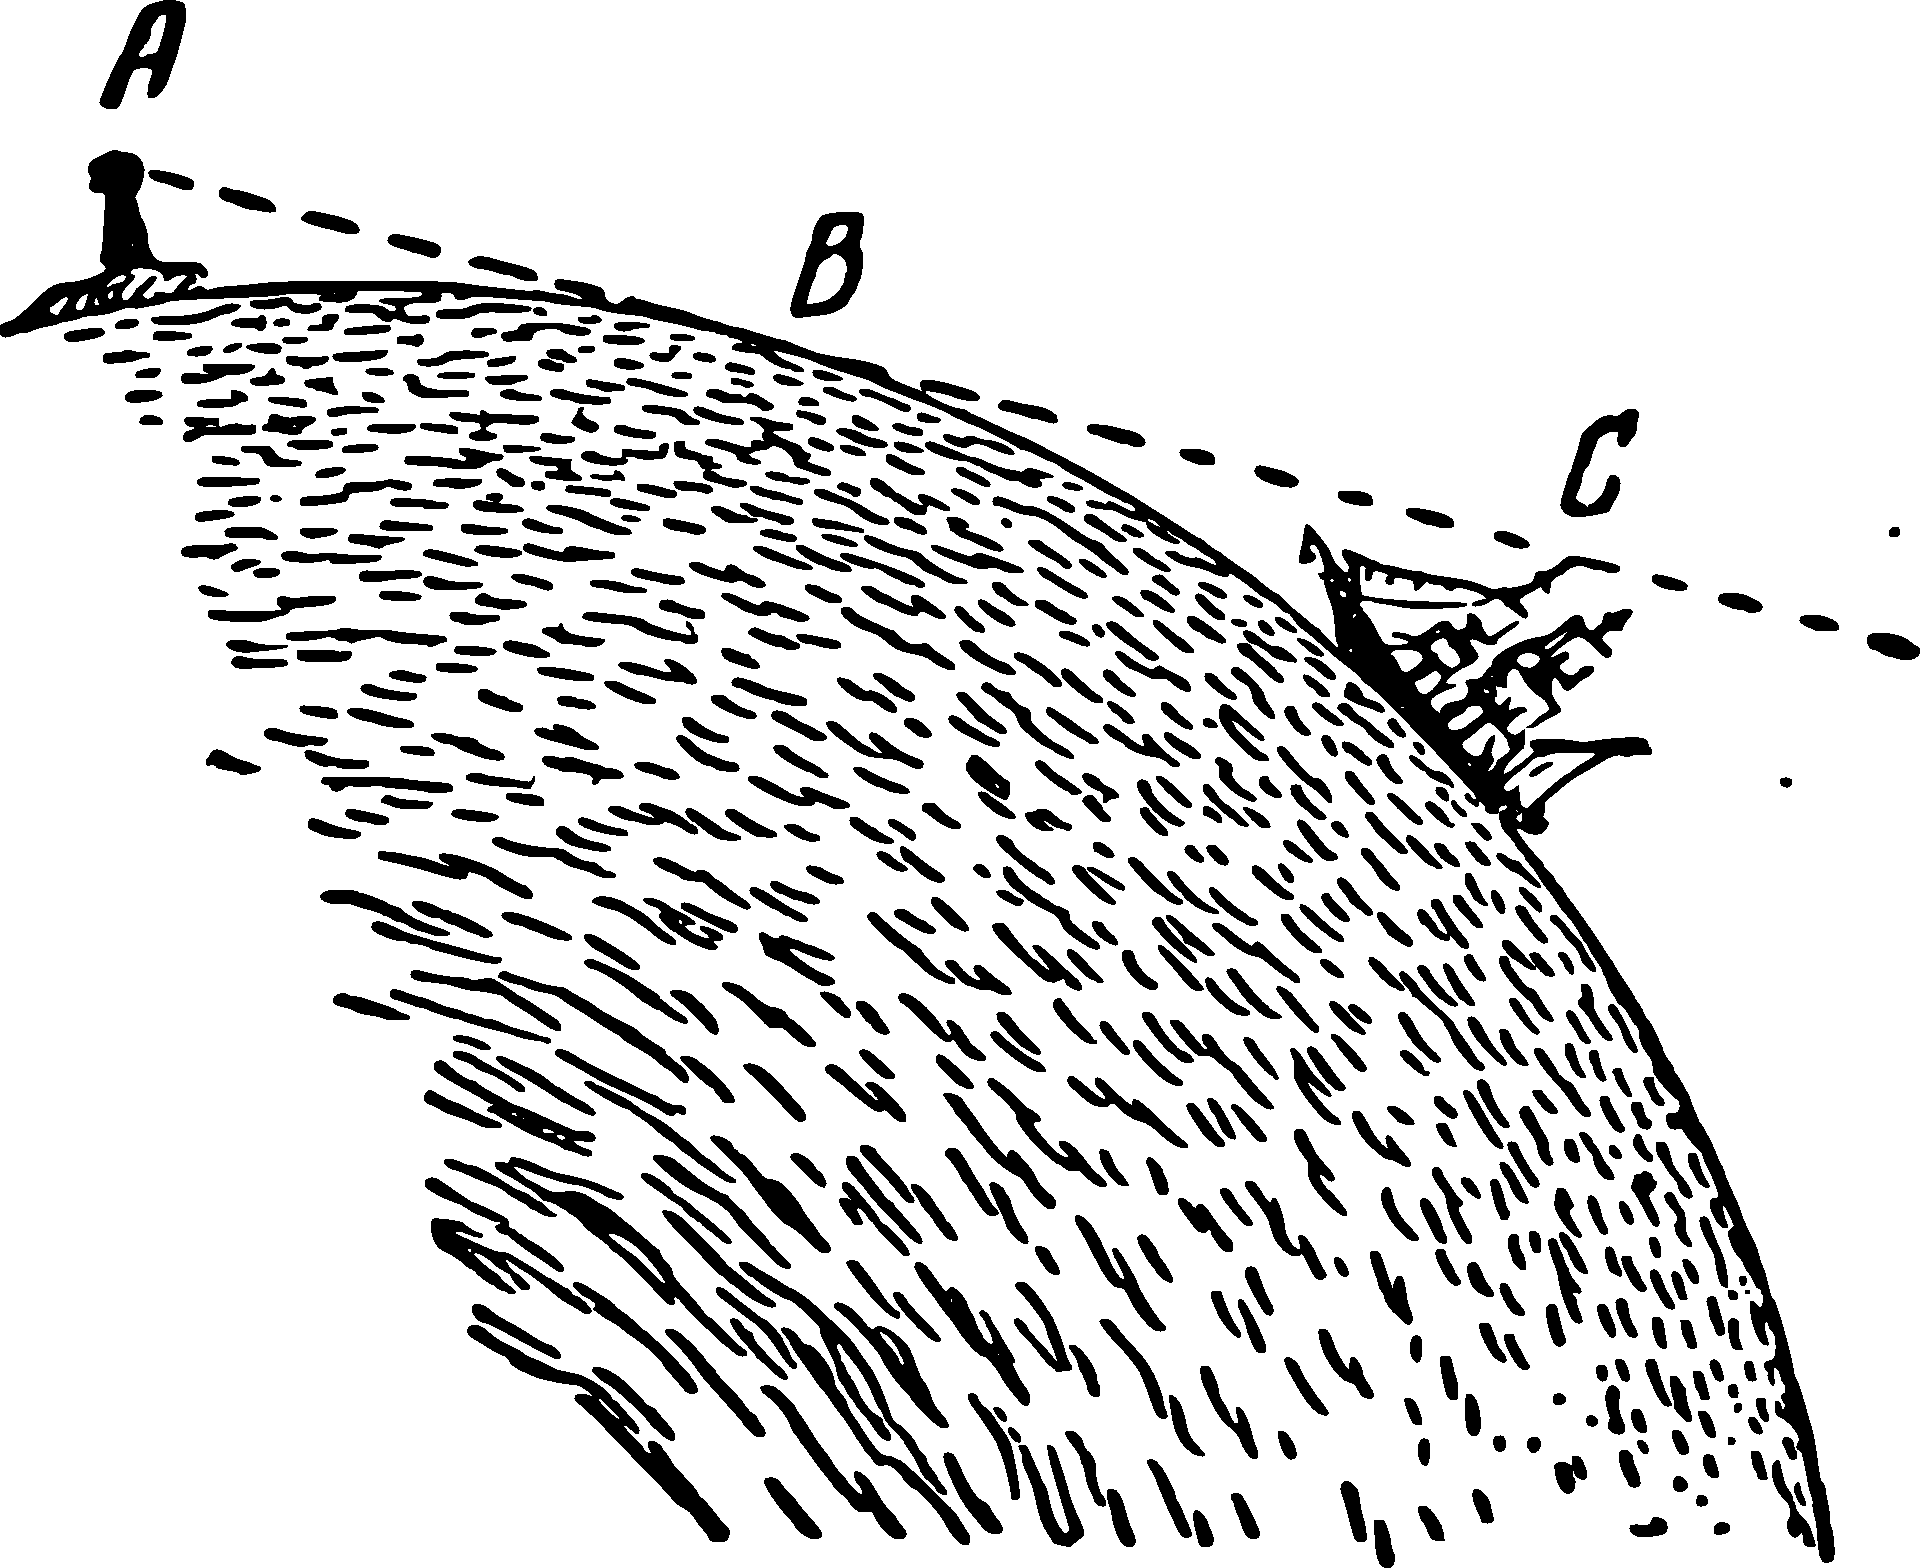
\includegraphics[width=0.8\textwidth]{figures/ch-06/fig-105.pdf}
\sidecaption{Lighthouse problems.\label{fig-105}}
\end{figure}



\ans From \figr{fig-105}, it can be seen that the problem reduces to calculating the length of the straight line $AC$, composed of two parts, $AB$ and $BC$.

Part $AB$ is the horizon distance of the lighthouse at a height above the ground of 40 meters, and $BC$ is the horizon distance of the ``mastman'' at a height of 10 meters. Therefore, the required distance is
\begin{equation*}%
113 \sqrt{0.04} + 113 \sqrt{0.01} = 113\sqrt{0.2 + 0.01} = \SI{34}{\kilo\meter}.
\end{equation*}

\ques What part of this lighthouse will be visible to the same ``mastman'' from a distance of \SI{30}{\kilo\meter}?


\ans From \figr{fig-105}, the solution of the problem is clear: first, it is necessary to calculate the length of $BC$, then subtract the obtained result from the total length of $AC$, i.e., from 30 km, to find the distance $AB$. Knowing $AB$, we will calculate the height from which the horizon distance is equal to $AB$. Let's perform all these calculations:
\begin{align*}%
BC & = 113\sqrt{0.01} - \SI{11.3}{\kilo\meter};\\
30 - 11.3 & = \SI{18.7}{\kilo\meter}\\
\text{height} & = \frac{18.7^{2}}{2R} = \frac{350}{12800} = \SI{0.027}{\kilo\meter}.
\end{align*}
So, from a distance of \SI{30}{\kilo\meter}, \SI{27}{\meter} of the lighthouse's height remains invisible; only \SI{13}{\meter} is visible. 

\section{Lightning Problem}
\label{sec-6.8}

\ques A lightning struck above your head at a height of \SI{1.5}{\kilo\meter}. At what distance from your location could the lightning still be visible?

\begin{figure}[h!]
\centering
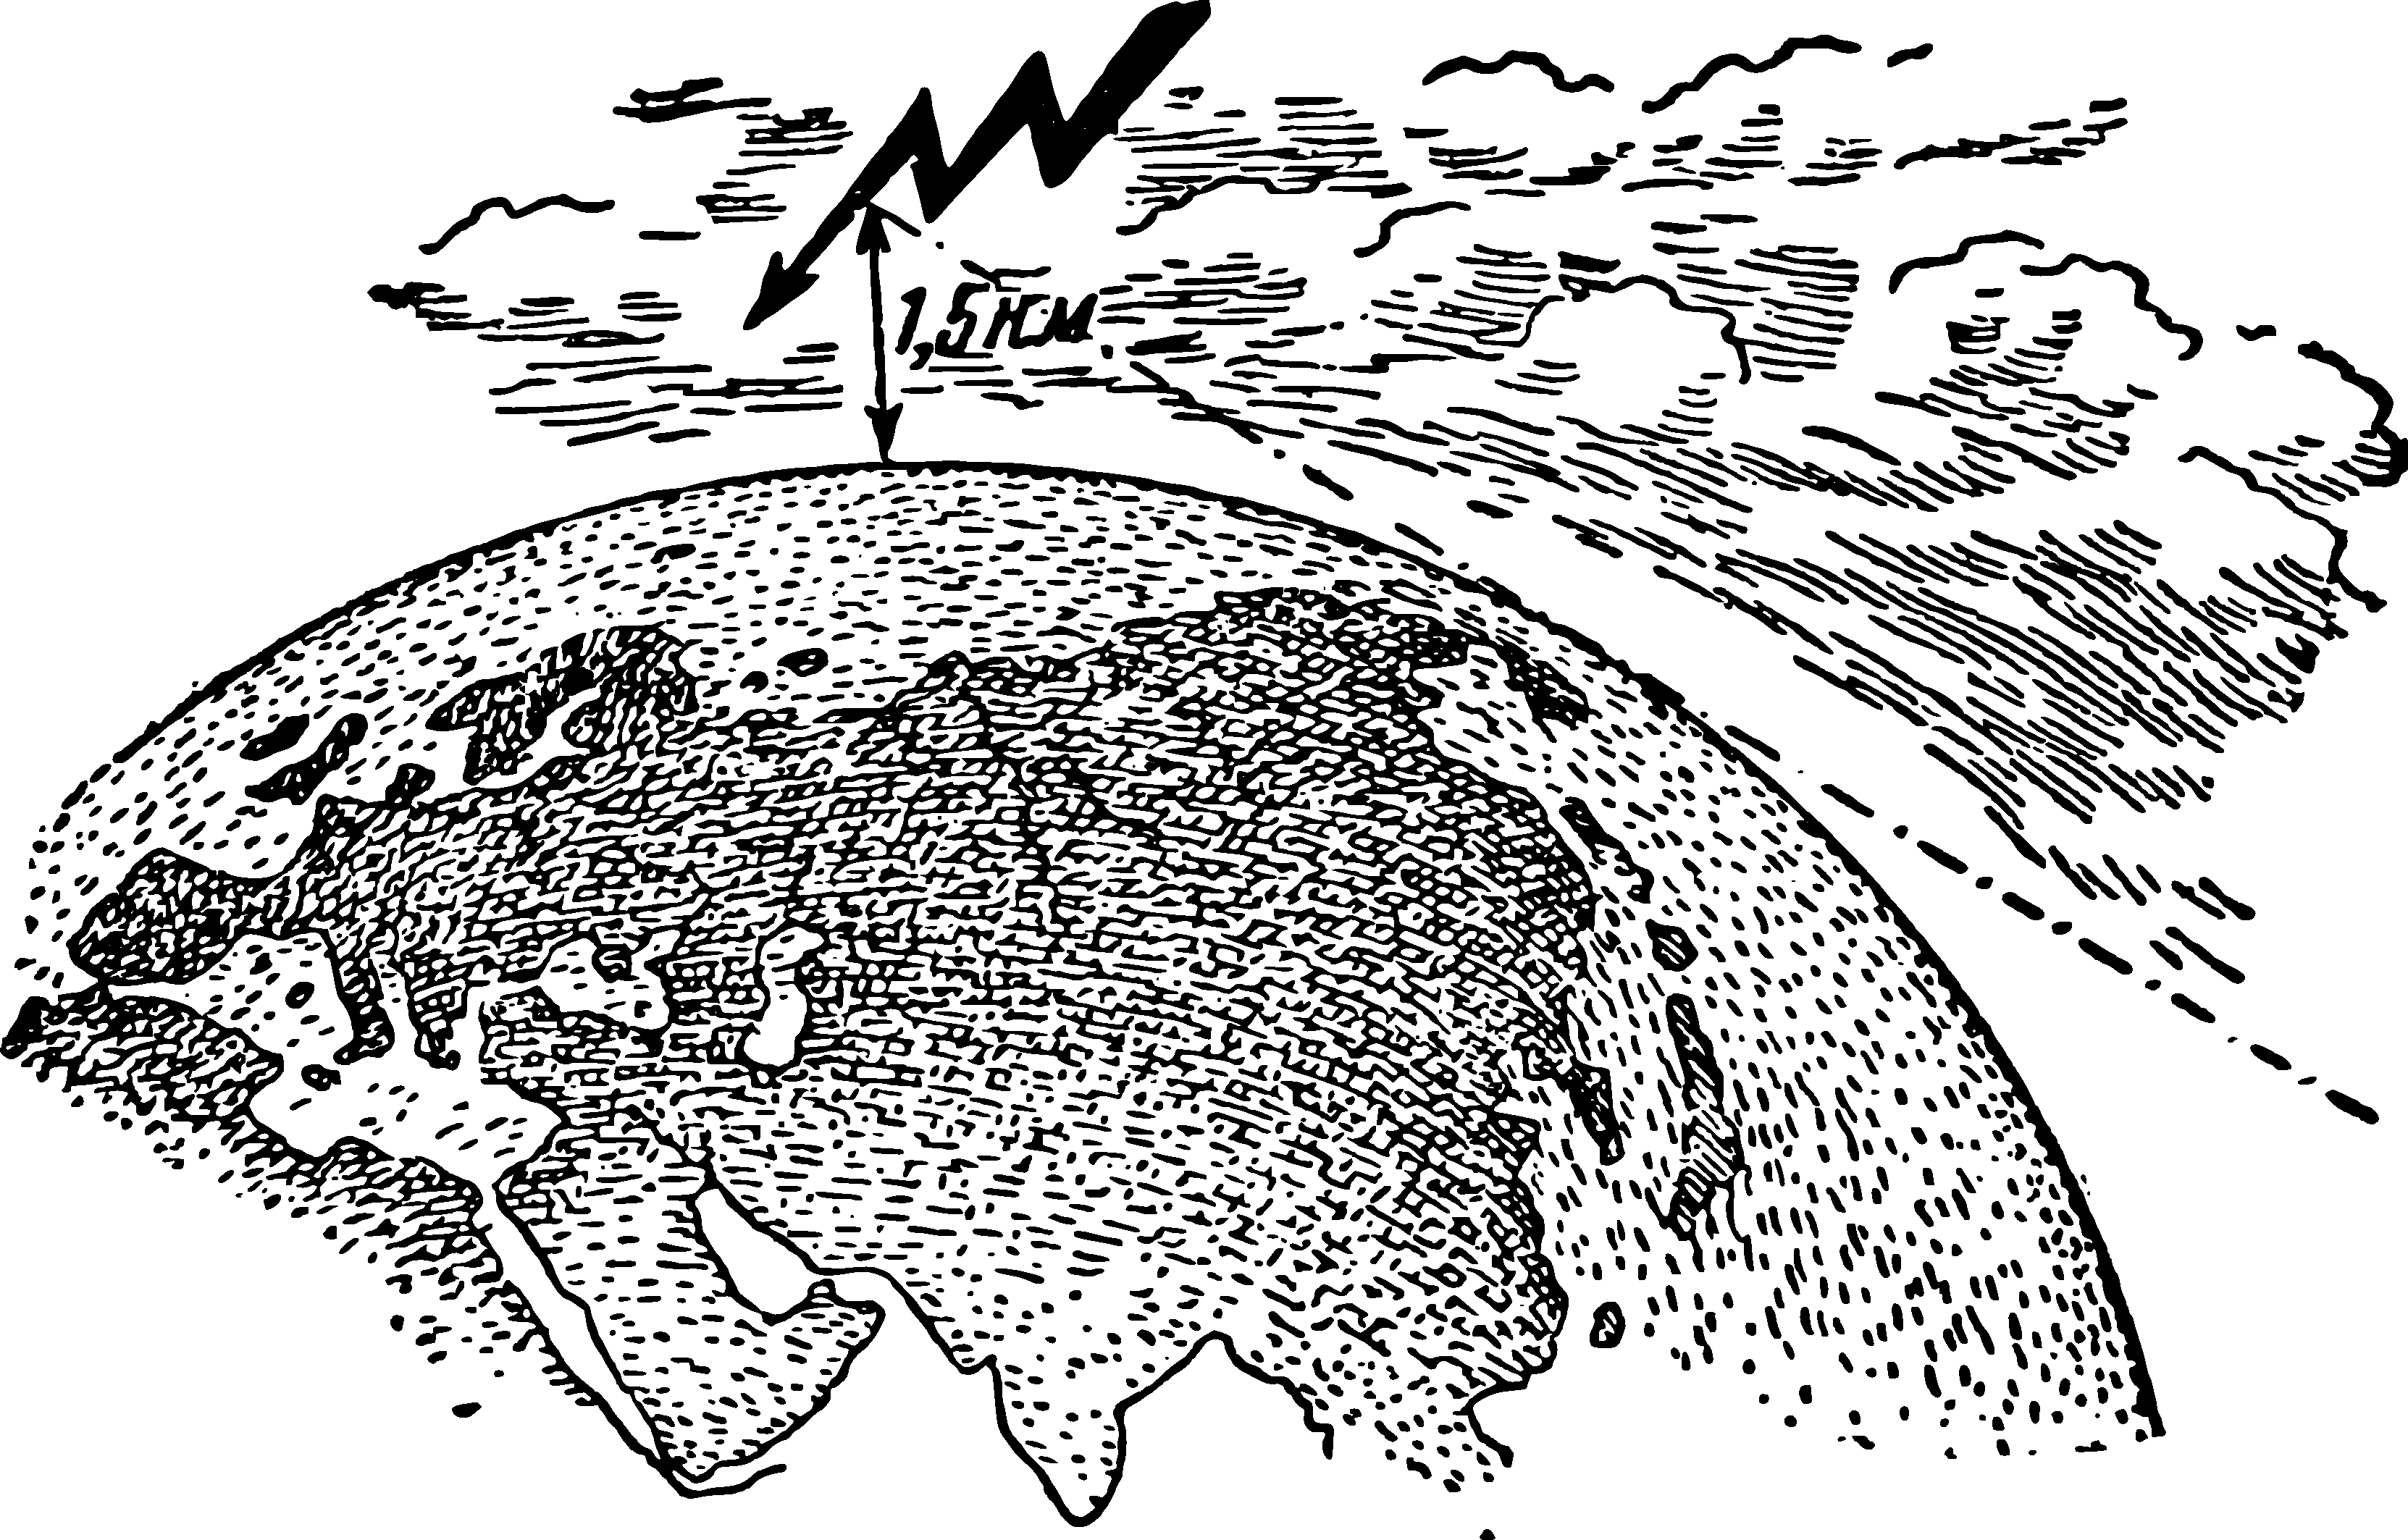
\includegraphics[width=0.8\textwidth]{figures/ch-06/fig-106.pdf}
\sidecaption{Lightning problem.\label{fig-106}}
\end{figure}



Solution: We need to calculate (see \figr{fig-106}) the horizon distance for a height of \SI{1.5}{\kilo\meter}. It equals 
\begin{equation*}%
113\sqrt{1.5} = \SI{138}{\kilo\meter}. 
\end{equation*}
Thus, if the terrain is flat, the lightning would have been visible to a person whose eyes are at ground level at a distance of \SI{138}{\kilo\meter} (with a 6\% correction, it would be \SI{146}{\kilo\meter}). At points \SI{146}{\kilo\meter} away, it would have been visible right at the horizon, and since sound does not carry over such distances, it would have been observed here as sheet lightning -- lightning without thunder.

\section{Sailboat Problem}
\label{sec-6.9}

\ques You are standing on the shore of a lake or sea, right by the water, observing a sailboat sailing away from you. You know that the top of the mast rises \SI{6}{\meter} above sea level. At what distance from you will the sailboat start to appear to descend into the water (i.e., beyond the horizon), and at what distance will it disappear completely?

\ans The sailboat will start to disappear below the horizon (see \figr{fig-100}) at point $B$ -- at the horizon distance for a person of average height, i.e., \SI{4.4}{\kilo\meter}. It will completely disappear below the horizon at a point where the distance from $B$ equals 
\begin{equation*}%
113\sqrt{0.006} = \SI{8.7}{\kilo\meter}. 
\end{equation*}
Thus, the sailboat will disappear below the horizon at a distance from the shore of 
\begin{equation*}%
4.4 + 8.7 = \SI{13.1}{\kilo\meter}. 
\end{equation*}


\section{Horizon on the Moon}
\label{sec-6.10}

\ques So far, all our calculations have related to the Earth's sphere. But how would the horizon distance change if the observer were on another planet, for example, on one of the plains of the Moon?


\ans The problem is solved using the same formula; the horizon distance equals $\sqrt{2Rh}$, but in this case, instead of $2R$, we need to substitute the diameter of the Moon's sphere. Since the diameter of the Moon is \SI{3500}{\kilo\meter}, then at an eye elevation of \SI{1.5}{\meter} above the ground, we have:
\begin{equation*}%
\text{horizon distance} = \sqrt{3500 \times 0.0015} = \SI{2.3}{\kilo\meter}.
\end{equation*}
On the lunar plain, we would see into the distance only up to \SI{2.3}{\kilo\meter}.


\section{In the Lunar crater}
\label{sec-6.11}

\ques Observing the Moon through even modest-sized telescopes, we see numerous so-called ring mountains -- formations that do not exist on Earth. One of the greatest ring mountains -- `` Copernicus Crater'' -- has an outer diameter of \SI{124}{\kilo\meter} and an inner diameter of \SI{90}{\kilo\meter}. The highest points of the ring wall rise above the inner crater floor by \SI{1500}{\meter}. But if you were in the middle part of the inner crater, would you see this ring wall from there?

\ans To answer the question, we need to calculate the horizon distance for the top of the wall, i.e., for a height of \SI{1.5}{\kilo\meter}. It equals on the moon to $\sqrt{3500 \times 1.5} = \SI{23}{\kilo\meter}$. Adding the horizon distance for an average-height person, we get the distance at which the ring wall is hidden below the observer's horizon:
\begin{equation*}%
23 + 2.3 \approx \SI{25}{\kilo\meter}.
\end{equation*}
And since the centre of the wall is \SI{45}{\kilo\meter} away from its edges, it is impossible to see this wall from the centre --unless you climb the slopes of the central mountains, rising on the floor of this crater to a height of \SI{600}{\meter}.\sidenote[][-1cm]{See the book by the same author \emph{Astronomy for Entertainment}, Chapter 3, article \emph{Lunar Landscapes}.}

\section{On Jupiter}
\label{sec-6.12}

\ques How far is the horizon on Jupiter, whose diameter is 11 times greater than Earth's?

\ans If Jupiter is covered by a solid crust and has a flat surface, then a person transported to its plain could see into the distance for:
\begin{equation*}%
\sqrt{11 \times 12800 \times 0.0016} = \SI{14.4}{\kilo\meter}.
\end{equation*}

\section*{For independent exercises}
\begin{enumerate}
\item Calculate the horizon distance for the periscope of a submarine, raised above the calm surface of the sea by \SI{30}{\centi\meter}.

\item How high should a pilot fly over Lake Ladoga to see both shores, separated by a distance of \SI{210}{\kilo\meter}?

\item How high should a pilot fly between Leningrad and Moscow to see both cities at once? The distance between Leningrad and Moscow is \SI{640}{\kilo\meter}.
\end{enumerate}


\begin{center}
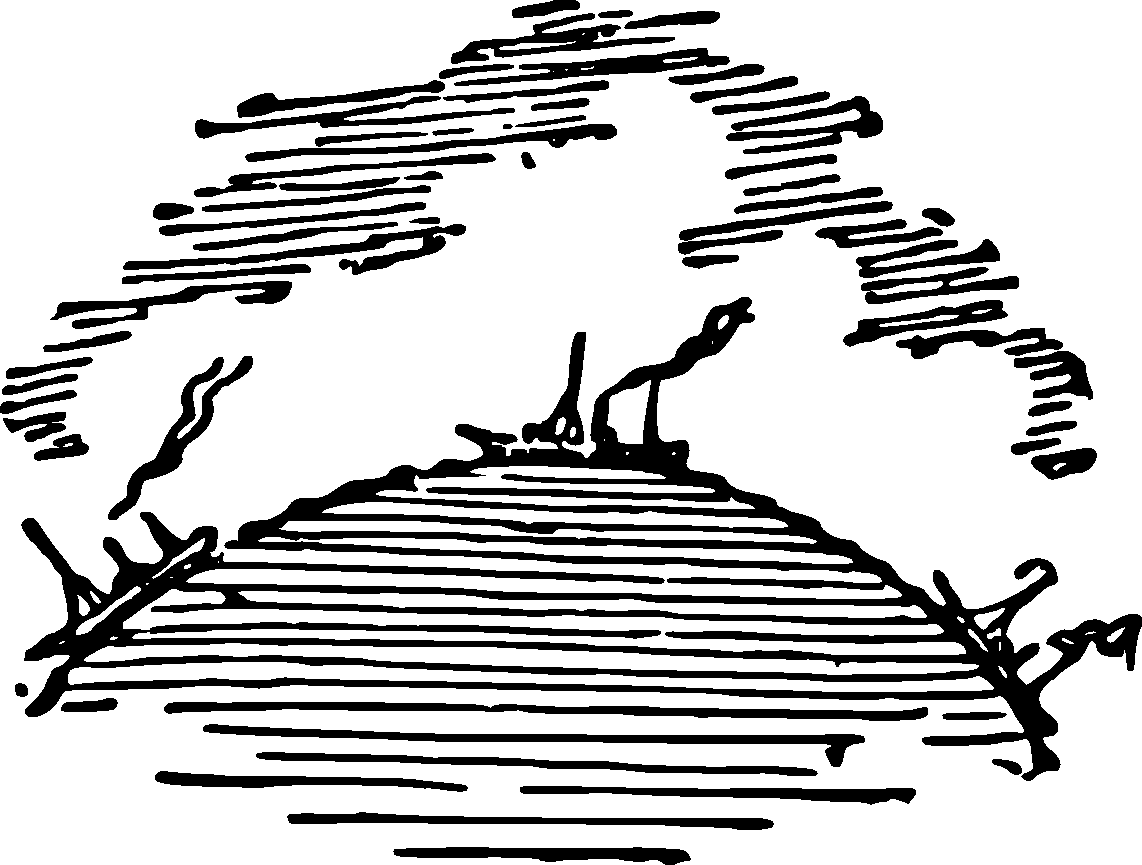
\includegraphics[width=0.3\textwidth]{figures/ch-06/fig-ch-06-tail.pdf}
\end{center}


















